% =====================================================================
%  University Course Timetabling System
%  Semester VII B.Tech. Project Report  --  Project "taasika-v3"
%  COEP Technological University, Pune
%
%  Formatting follows BTechProjectCSE_Latex_Template_2026-27
%  (report class, 12 pt, one column, 1.5 line spacing, template margins,
%  template title page, certificate, plagiarism page, front-matter order,
%  plain bibliography after the appendices).
% =====================================================================
\documentclass[a4paper,12pt,onecolumn]{report}

\usepackage[T1]{fontenc}
\usepackage[utf8]{inputenc}
\usepackage{lmodern}
\usepackage{microtype}
\usepackage{graphicx}
\usepackage{booktabs}
\usepackage{longtable}
\usepackage{array}
\usepackage{multirow}
\usepackage{tabularx}
\usepackage{caption}
\usepackage{float}
\usepackage{enumitem}
\usepackage{titlesec}
\usepackage{etoolbox}
\usepackage{listings}
\usepackage{xcolor}
\usepackage{amsmath}
\usepackage{amssymb}
\usepackage{tikz}
\usepackage{pgfplots}
\usepackage{pgfplotstable}
\usepackage[hidelinks]{hyperref}

% ------------------------------------------------------- page layout
% Template margins: left 2.5 cm, top 2 cm, right 2 cm, bottom 2 cm,
% 0.5 cm binding offset.
\usepackage[a4paper,left=2.5cm,top=2cm,right=2cm,bottom=2cm,bindingoffset=0.5cm]{geometry}

% ------------------------------------------------------- body text
% Template: Computer Modern, 12 pt, line spacing 1.5.
\linespread{1.5}

% The body is 12 pt as the template requires. Footnote-size and smaller
% text (tables, captions, listings, figure labels) keeps the absolute sizes
% the tables and figures were drawn for.
\makeatletter
\renewcommand\small{\@setfontsize\small\@ixpt{11}}
\renewcommand\footnotesize{\@setfontsize\footnotesize\@viiipt{9.5}}
\renewcommand\scriptsize{\@setfontsize\scriptsize\@viipt\@viiipt}
\renewcommand\tiny{\@setfontsize\tiny\@vpt\@vipt}

% 1.5 spacing applies to running text only. Tables, listings and
% drawings are set single-spaced so they keep their designed height.
\newcommand{\singlespacedblock}{\def\baselinestretch{1}\@currsize}
\AtBeginEnvironment{tabular}{\singlespacedblock}
\AtBeginEnvironment{tabularx}{\singlespacedblock}
\AtBeginEnvironment{longtable}{\singlespacedblock\small}
\AtBeginEnvironment{lstlisting}{\singlespacedblock}
\AtBeginEnvironment{tikzpicture}{\singlespacedblock}
\makeatother

% At 12 pt, long file names and paths in \texttt no longer fit on a line.
% Allow line breaks after "/" and "_" inside \texttt (formatting only).
\makeatletter
{\catcode`\/=\active \catcode`\-=\active \catcode`\.=\active
 \gdef\texttt@breaks{\catcode`\/=\active \catcode`\-=\active \catcode`\.=\active
   \def/{\char`\/\allowbreak}\def-{\char`\-\allowbreak}\def.{\char`\.\allowbreak}%
   \def\_{\textunderscore\allowbreak}}}
\setlength{\tabcolsep}{5pt}
\DeclareRobustCommand{\texttt}{\begingroup\texttt@breaks\texttt@aux}
\newcommand{\texttt@aux}[1]{{\ttfamily #1\/}\endgroup}
\makeatother

% The wide definition display in Appendix C is set one size smaller.
\AtBeginEnvironment{align*}{\small}

\DeclareCaptionFont{singlesmall}{\small\def\baselinestretch{1}\small}
\captionsetup{font=singlesmall,labelfont=bf,width=0.92\textwidth}

% ------------------------------------------------------- numbering
% Content is organised in sections (not chapters). Number them 1, 2, 3...
% and, in the appendices, A, B, C...
\renewcommand{\thesection}{\arabic{section}}

% The unnumbered "Abstract" heading is centred and large, as in the
% template's abstract page.
\titleformat{name=\section,numberless}[block]{\normalfont\Large\bfseries\centering}{}{0pt}{}

\emergencystretch=3em
\tolerance=2000

% ------------------------------------------------------- styling
\pgfplotsset{compat=1.18}
\usetikzlibrary{shapes.geometric,arrows.meta,positioning,calc,fit,backgrounds,decorations.pathreplacing}

\definecolor{coepblue}{RGB}{20,60,110}
\definecolor{lstbg}{RGB}{247,247,247}
\definecolor{lstkw}{RGB}{20,60,110}
\definecolor{lstcm}{RGB}{110,110,110}

\lstset{
  basicstyle=\ttfamily\scriptsize,
  backgroundcolor=\color{lstbg},
  keywordstyle=\color{lstkw}\bfseries,
  commentstyle=\color{lstcm}\itshape,
  stringstyle=\color{black},
  frame=single,
  framesep=4pt,
  rulecolor=\color{gray!40},
  breaklines=true,
  breakatwhitespace=true,
  columns=fullflexible,
  showstringspaces=false,
  numbers=left,
  numberstyle=\tiny\color{gray},
  numbersep=7pt,
  captionpos=b,
  xleftmargin=16pt,
}
\lstdefinestyle{plainlst}{numbers=none,xleftmargin=4pt}

% \todo{} -- visible placeholder for anything not yet verifiable
\newcommand{\todo}[1]{\textcolor{red!80!black}{\textbf{[TODO:} #1\textbf{]}}}

\newcolumntype{L}[1]{>{\raggedright\arraybackslash}p{#1}}
\newcolumntype{C}[1]{>{\centering\arraybackslash}p{#1}}

\setlist[itemize]{topsep=2pt,itemsep=1pt,parsep=0pt,leftmargin=1.4em}
\setlist[enumerate]{topsep=2pt,itemsep=1pt,parsep=0pt,leftmargin=1.6em}

\begin{document}

% Front matter is numbered in lowercase roman, as the template's own
% comment intends; main text restarts in arabic below.
\pagenumbering{roman}

% ================================================================ TITLE PAGE
%_____________________________________________________________________________________________
% Title page, following BTechProjectCSE_Latex_Template_2026-27/titlepage.tex
% MIS numbers and the guide's title are not in the repository; they are
% marked with \todo and must be filled in.
%_____________________________________________________________________________________________
\begin{titlepage}
\begin{center}
\LARGE{\bf{University Course Timetabling System\\}}
\Large{\bf{ B. Tech. Project Report\\}}
\Large{\em{Submitted by\\}}
\vspace{0.3cm}

\begin{tabular}{ l c c l }
\Large\bf{Mihir Shah}      & & & \Large\bf{612303118} \\[0.3cm]
\Large\bf{Riya Kulkarni}   & & & \Large\bf{612303151} \\[0.3cm]
\Large\bf{Ved Mundhada}    & & & \Large\bf{612303123} \\[0.3cm]
\Large\bf{Akshay Sathaye}  & & & \Large\bf{612303159} \\
\end{tabular}

\vspace{0.3cm}
\Large{Under the guidance of\\ }
\Large{\bf{Prof Abhijit A. M.}\\}
\Large{COEP Technological University, Pune\\}

\begin{figure}[h]
\centering

\includegraphics[width=5cm,height=5cm]{figures/COEP_Tech_University_Logo.jpg}
\end{figure}

\large{\bf{DEPARTMENT OF COMPUTER SCIENCE \& ENGINEERING}}\\
\Large{\bf{COEP TECHNOLOGICAL UNIVERSITY\\ (COEP TECH), PUNE - 5}}
\vfill
\large{\bf{November 2026}}
\end{center}
\end{titlepage}


% ================================================================ CERTIFICATE
%_____________________________________________________________________________________________
% Certificate page, following BTechProjectCSE_Latex_Template_2026-27/certi.tex
% MIS numbers are not in the repository and are marked with \todo.
%_____________________________________________________________________________________________
\thispagestyle{empty}
{
\linespread{2}\selectfont
\begin{center}
	\large{\bf{DEPARTMENT OF COMPUTER SCIENCE \& ENGINEERING,\\
	      COEP TECHNOLOGICAL UNIVERSITY, PUNE - 5\\}}
\end{center}

\vspace{20pt}

\begin{center}
	\Large{\bf{CERTIFICATE\\}}
\end{center}

\vspace{20pt}
}

\linespread{1.5}\selectfont
\large{
Certified that this project titled, ``University Course Timetabling System''
has been successfully completed by \\
\begin{center}
	\begin{tabular}{ l c c l }
	\Large\bf{Mihir Shah}      & & & \Large\bf{612303118} \\ [0.3cm]
	\Large\bf{Riya Kulkarni}   & & & \Large\bf{612303151} \\ [0.3cm]
	\Large\bf{Ved Mundhada}    & & & \Large\bf{612303123} \\ [0.3cm]
	\Large\bf{Akshay Sathaye}  & & & \Large\bf{612303159} \\
	\end{tabular}
\end{center}
and is approved for the partial fulfillment of the requirements for the degree of
``B. Tech. Computer Engineering''.
}



% ================================================ PLAGIARISM REPORT PAGE
\newpage
\thispagestyle{empty}
\vspace*{\fill}
\begin{center}
  \todo{Insert the scanned plagiarism-percentage page, signed by the Project Guide, here.}
\end{center}
\vspace*{\fill}

% ================================================================ ABSTRACT
\newpage
\section*{Abstract}
\addcontentsline{toc}{section}{Abstract}

University course timetabling is an NP-hard combinatorial optimisation problem in which classes,
instructors, student cohorts and rooms must be assigned to time slots subject to a large set of
hard and soft constraints. The Semester~VI phase of this project established that UniTime, an
open-source constraint-driven academic scheduling system, is able to express every scheduling
constraint identified at COEP Technological University without relaxation or external
post-processing. That phase was a feasibility study: it configured a local deployment and entered
representative test data, but it did not produce a timetable from institutional data.

The present phase, carried out under the project name \emph{taasika-v3}, converted that feasibility
result into a working system. A reproducible data pipeline was built that reads a snapshot of the
university's existing Taasika scheduling database and emits the sixteen ordered XML documents that
UniTime's Data Exchange interface requires, covering the academic session, curriculum structure,
rooms, instructors, course offerings, scheduling preferences and a simulated student body of
1{,}130 students with 9{,}148 section enrolments. Institution-specific rules---minor-degree and
open-elective time blocks, division and batch structure, and dynamic lunch breaks for both students
and instructors---were encoded as generated preference data rather than as manual edits. An
independent evaluation framework was written to score any exported timetable against the same input
data, because the solver's own quality report cannot be used to audit the solver.

Using this framework, the project established a result that the solver's internal counters had been
concealing. Several earlier runs reported zero student conflicts; each was traced to an artefact
rather than to a better timetable, the most common being UniTime silently re-sectioning students
between laboratory batches. Once student enrolments were pinned---by selecting
\emph{Enrolled Student Course Demands} and disabling student switching and re-sectioning---the final
solution scheduled 290 of 291 classes with no instructor and no room double-booking, a hard
feasibility score of 98.85 out of 100, and 40 of 1{,}130 students (3.54\,\%) carrying a timetable
clash, all of them first-year students in a single laboratory--lecture pairing.

A reinforcement-learning layer was also implemented, in which a policy selects among eight stock
CPSolver neighbourhood operators inside the existing search loop. The layer is complete and
instrumented, comprising 25 Java classes and 11 Python modules, and it never writes a placement
itself, so hard-constraint safety is unchanged. Its pre-registered control experiment, however,
answered the project's own research question in the negative: simply raising the solver's
student-conflict weight reduced the violation rate from 0.0414 to below 0.004 on the same instance,
clearing the 25\,\% improvement threshold that the learned policy was intended to achieve. No claim
is therefore made that the learned policy outperforms the baselines; the report states precisely
what was implemented, what was measured, and what remains a hypothesis.


% ================================================ CONTENTS AND LISTS
\newpage
\tableofcontents

\listoftables
\addcontentsline{toc}{chapter}{List of Tables}

\listoffigures
\addcontentsline{toc}{chapter}{List of Figures}

%_____________________________________________________________________________________________
% List of Symbols (the template provides an empty heading; the entries below
% are the symbols this report defines, with the section that defines them).
%_____________________________________________________________________________________________
\chapter*{List of Symbols}

\begin{center}
\begin{tabular}{@{}l p{8.2cm} l@{}}
\toprule
Symbol & Meaning & Section \\
\midrule
$\omega$ & current (partial) timetable in Iterative Forward Search & 3 \\
$\sigma$ & best timetable found so far & 3 \\
$S$ & set of students in the enrolment data & Appendix C \\
$A$ & set of assigned classes in a solution & Appendix C \\
$E(s)$ & assigned classes student $s$ is enrolled in & Appendix C \\
$\mathrm{ov}(c_1,c_2)$ & classes $c_1$ and $c_2$ overlap for a student & Appendix C \\
$C$ & student violation rate: conflicted students over students enrolled in at least two classes & 10, Appendix C \\
$C_{\mathrm{checker}}$ & conflicted students over all students & Appendix C \\
$H$ (checks) & set of hard checks in the aggregate score & Appendix C \\
$P$ & set of preference checks in the aggregate score & Appendix C \\
$r$ & pass rate of one check, in $[0,1]$ & Appendix C \\
$K$ & solver iterations per reinforcement-learning macro-step ($K=50$) & 11 \\
$\Phi$ & potential used for reward shaping & 11 \\
$U$ & unassigned fraction of classes & 11 \\
$H$ (violations) & number of hard violations & 11 \\
$O$ & normalised soft objective & 11 \\
\bottomrule
\end{tabular}
\end{center}

\addcontentsline{toc}{chapter}{List of Symbols}

\newpage
\pagenumbering{arabic}

% ================================================================ SECTIONS
\section{Introduction}
\label{sec:intro}

The problem of Course Timetabling in a university is the problem of assigning many classes with a set of rooms, teachers and time constraints to a weekly timetable in a grid, under many different hard and soft constraints. The problem is NP-hard, which means that we do not know any polynomial time exact solution or have practical systems that use heuristic or metaheuristic search~\cite{schaerf1999survey,muller2007}.

COEP Technological University offers a challenging example of this. The Department of Computer Engineering has four undergraduate years and a postgraduate programme that each consist of lecture divisions and then laboratory batches, with departmental electives, minor degree courses offered by other disciplines, open electives and reserved first-year batches. Laboratory sections are parallel courses, courses are parallel lectures, and a scheduling unit is not the course itself, but the section of it, to the extent that the scheduling unit is fit to be used, or not, depends on the relations between the sections, not the course itself.

\subsection{The school values that were set by Semester~VI}

The previous step in this project was to assess UniTime, an academic scheduling system developed as an open source, web-based platform using the CPSolver constraint library, for suitability as a platform. It installed the system in its own environment and loaded representative test data into it both via the web interface and via the XML import feature, and translated the institution's scheduling rules into UniTime's constraint model. The conclusion was that all the constraints found by the team were representable in that model and none of the constraints needed to be relaxed or post-processed externally.

Upon completion of Semester~VI, there was no institutional data, no real solution found from the course structure, and no measure for the quality of the solution. All the data pipeline, student records, and the instructor-facing interface were all described in the future tense.

\subsection{There are 1.2 credits earned for Semester~VII}

The current phase is the \emph{taasika-v3}, which addresses that. The entire work is organized in five contributions, each of which is reported along with the evidence that supports it:

\begin{enumerate}
  \item \textbf{A reproducible Taasika\,$\rightarrow$\,UniTime data pipeline.} Eight Python
    generators read a snapshot of the university's existing Taasika scheduling database and emit
    the sixteen ordered XML documents that UniTime's Data Exchange interface consumes, followed by
    three validators and an archive step, behind a single command
    (Section~\ref{sec:pipeline}).
  \item \textbf{Institution-specific constraints encoded as data.} Minor-degree and open-elective
    block times, division and batch structure, elective spread, and dynamic lunch breaks for
    students and instructors are generated into the preference file and solver configuration rather
    than entered by hand (Section~\ref{sec:constraints}).
  \item \textbf{An unbiased assessment system.} Because a solver cannot be audited with its own
    counters (Section~\ref{sec:evaluation}), a 1{,}044-line evaluator is used to score any exported
    timetable against the same input XML with 10 hard checks, 3 preference checks and a set of
    efficiency metrics.
  \item \textbf{The accurate description of the solution quality.} A number of configurations
    experienced no student conflict reported, all of which were found to be artefacts. For the last
    30 weeks, student enrolments have been fixed, and double-bookings of instructors and rooms have
    been avoided: 290 of 291 classes have been scheduled in a way that avoids instructor or room
    double-booking; 40 of 1{,}130 students are in conflict (Section~\ref{sec:experiments}).
  \item \textbf{Reinforcement learning for the solver search.} A policy is a choice from eight
    neighbourhood operators for the CPSolver, which are implemented within the search loop. The
    layer is implemented and instrumented, and is the result of a negative answer to the research
    question (Section~\ref{sec:rl}).
\end{enumerate}

The project is referred to throughout as \emph{taasika-v3}. The source repository retains an earlier
name, \texttt{coep-unitime-pilot}, which should be read as a historical artefact rather than as a
description of the current scope.

\section{Problem Definition}
\label{sec:problem}

The objective is to produce, automatically and reproducibly, a weekly timetable for the Department
of Computer Engineering that satisfies every mandatory institutional rule and violates as few
preferential rules as possible. A comprehensive review of the literature confirms that constraint
programming is the predominant methodology for this class of problem, owing to its ability to model
mandatory and preferential requirements in a single framework~\cite{schaerf1999survey,muller2007}.

\subsection{Scheduling model}

In the CPSolver course-timetabling model the decision variable is a \emph{class} (a single lecture,
laboratory or tutorial section), and its value is a \emph{placement}: a starting time together with
the room or rooms in which the class meets. Students are not decision variables. A student's
timetable is a consequence of the placements chosen for the classes that student is enrolled in, and
the cost of two classes overlapping for a shared cohort is priced through a joint-enrolment
constraint between those two classes. This distinction matters for everything that follows: the
solver can only improve a student's timetable by moving a class, or---if it is permitted to do
so---by moving the student into a different section. Student sectioning is otherwise a problem in its own right~\cite{muller2010sectioning}.

\subsection{Hard and soft constraints}

Hard constraints must hold in any acceptable timetable:

\begin{itemize}
  \item no room hosts two classes at overlapping times;
  \item no instructor teaches two classes at overlapping times;
  \item a class is placed only in a room whose capacity meets its enrolment limit and whose type
    and equipment suit the subpart;
  \item every class respects the meeting pattern declared for its subpart (for example
    $2\times120$ minutes) and the date pattern of the term;
  \item rooms are used only when available, and weekends are excluded.
\end{itemize}

Soft constraints express quality rather than legality: preferred rooms and time windows, balanced
instructor load, limited back-to-back teaching, minimised travel between buildings, a protected
lunch window, and---the criterion this report treats as primary---the number of students whose
personal timetable contains an overlap. Soft requirements enter as weighted criteria rather than as further hard constraints~\cite{rudova2003soft}.

\subsection{Student conflicts and the measurement problem}

Two classes conflict for a student if and only if they share a day, their slot intervals overlap,
and, when both carry date patterns, they share at least one active week. Intervals that merely touch
at an endpoint do not conflict, and room and instructor are irrelevant to the test. This rule is
implemented identically in three places that were used during the project---CPSolver's own time
representation, the Java conflict oracle written for the learning layer, and the Python evaluator
described in Section~\ref{sec:evaluation}---and the agreement between them is reported in
Section~\ref{sec:evaluation}.

The central difficulty of this phase was not producing a feasible timetable; coverage, room and
instructor feasibility were reached early. The difficulty was that student-conflict counts could not
be trusted. Three mechanisms independently drive the reported figure to zero without improving any
student's timetable:

\begin{enumerate}
  \item \textbf{Re-sectioning.} If student switching and initial sectioning are enabled, UniTime
    moves students between parallel laboratory batches until the overlaps disappear. The timetable
    is unchanged; the cohort structure of the institution is silently discarded.
  \item \textbf{An empty student population.} Under the \emph{Projected Student Course Demands}
    setting, and with no last-like enrolment data in the session, the solver loads zero students and
    reports a conflict count of zero over an empty denominator.
  \item \textbf{A denominator mismatch.} A conflict rate computed over the students who carry
    enrolments in a solver export is not comparable to one computed over every simulated student in
    the source data, and the two populations differed by several hundred students across the
    instances used in this project.
\end{enumerate}

The problem addressed in Sections~\ref{sec:evaluation} and~\ref{sec:experiments} is therefore stated
as two objectives rather than one: produce a feasible timetable, and establish a measurement of
student conflicts that cannot be satisfied by any of the three mechanisms above.

\section{Overview of UniTime and CPSolver}
\label{sec:unitime}

\subsection{The UniTime system}

UniTime is a comprehensive, open-source academic scheduling system released under the Apache
License, Version 2.0, and maintained as a sponsored project of the Apereo Foundation. It is
web-based, implemented in Java, and deployed at large institutions worldwide, including Purdue
University~\cite{rudova2011complex}. Later accounts of the same system cover elective courses and
multiple sections~\cite{muller2016curriculum}. The system comprises four integrated components: course timetabling, examination
timetabling, student scheduling, and event management. Only the first is used in this project,
although the data model shared by all four determines the structure of the import files described
in Section~\ref{sec:pipeline}.

Within UniTime a course is modelled hierarchically. A \emph{course offering} belongs to an
\emph{instructional offering}, which carries one or more \emph{configurations}; a configuration
contains \emph{scheduling subparts} (for example a lecture subpart and a laboratory subpart); and
each subpart contains the individual \emph{classes} that are actually placed in the timetable. A
class inherits its permitted meeting patterns from its subpart. This hierarchy is what allows a
course with joint lectures and parallel laboratory batches to be represented as a single offering,
and it is the reason the institution's division-and-batch structure maps onto UniTime without
distortion~\cite{murray2007modeling}.

\subsection{The constraint solver}

The embedded solver is CPSolver~\cite{cpsolver}, a local-search framework with constraint-programming primitives,
distributed under the GNU LGPL. It won two tracks of the International Timetabling Competition 2007
and reached the final in all three~\cite{muller2009itc,muller2025itc}. In the course-timetabling model the variable is a class, the
value is a placement of time and room, and the objective is a weighted sum of soft-constraint
criteria.

\subsection{Iterative Forward Search}

The solver is built on Iterative Forward Search (IFS)~\cite{muller2004}. IFS belongs to the family
of local-search methods, but differs from classical local search in that it operates over feasible
yet potentially \emph{incomplete} solutions: some classes may remain unassigned, but every hard
constraint holds for the classes that are assigned. Intermediate solutions are therefore always
interpretable and actionable by a human scheduler, in contrast to complete-but-infeasible solutions
produced by unconstrained search.

From an initial timetable $\omega$, each iteration selects a class and a placement, removes the
assignments that hard-conflict with it, and installs the new one. The best timetable seen,
$\sigma$, is kept and returned at the end, so the search can be stopped and resumed from any
feasible timetable. Listing~\ref{lst:ifs} states the algorithm; Figure~\ref{fig:solverloop} is the
same loop as it actually runs, including the distinction between proposing a move and committing
it. The learning layer of Section~\ref{sec:rl} replaces only the \emph{Propose move} box. That step
draws one assignment from the neighbourhood of the current one~\cite{muller2005thesis}. Later
changes to the competition solver's time changes, room changes and swaps are described
in~\cite{muller2016evolution}.

\begin{lstlisting}[style=plainlst,caption={Iterative Forward Search},label={lst:ifs}]
function IFS(omega):
    sigma = omega
    while canContinue(omega) do:
        v     = selectVariable(omega)            // select a class
        d     = selectValue(omega, v)            // select a placement
        gamma = hardConflicts(omega, v/d)        // conflicting assignments
        omega = (omega \ gamma) union {v/d}      // remove conflicts, assign
        if better(omega, sigma) then
            sigma = omega                        // update best solution
    end while
    return sigma
end function
\end{lstlisting}

\begin{figure}[H]
\centering
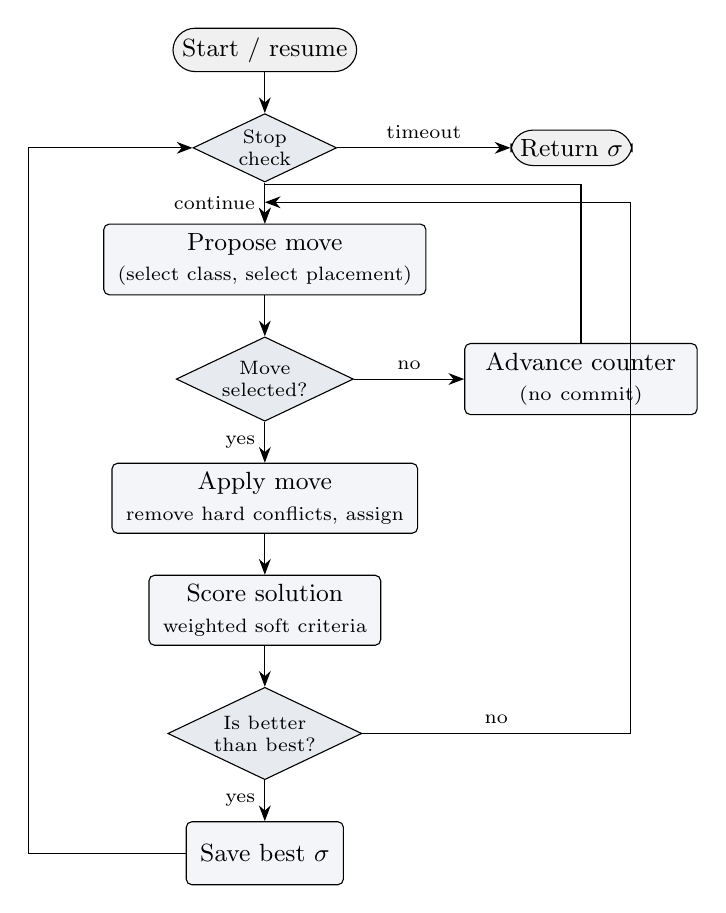
\begin{tikzpicture}[
  node distance=5.2mm and 8mm,
  box/.style={draw,rounded corners=2pt,align=center,font=\small,minimum height=8mm,inner xsep=5pt,fill=coepblue!5},
  dec/.style={draw,diamond,aspect=2.1,align=center,font=\scriptsize,inner sep=1pt,fill=coepblue!10},
  term/.style={draw,rounded corners=8pt,align=center,font=\small,fill=gray!12},
  ar/.style={-{Stealth[length=2mm]}}
]
\node[term] (start) {Start / resume};
\node[dec, below=of start] (stop) {Stop\\check};
\node[box, below=of stop] (prop) {Propose move\\{\scriptsize(select class, select placement)}};
\node[dec, below=of prop] (sel) {Move\\selected?};
\node[box, below=of sel] (apply) {Apply move\\{\scriptsize remove hard conflicts, assign}};
\node[box, below=of apply] (score) {Score solution\\{\scriptsize weighted soft criteria}};
\node[dec, below=of score] (better) {Is better\\than best?};
\node[box, below=of better] (save) {Save best $\sigma$};
\node[term, right=22mm of stop] (end) {Return $\sigma$};
\node[box, right=14mm of sel, text width=26mm] (adv) {Advance counter\\{\scriptsize (no commit)}};

\draw[ar] (start) -- (stop);
\draw[ar] (stop) -- node[left,font=\scriptsize]{continue} (prop);
\draw[ar] (stop) -- node[above,font=\scriptsize]{timeout} (end);
\draw[ar] (prop) -- (sel);
\draw[ar] (sel) -- node[left,font=\scriptsize]{yes} (apply);
\draw[ar] (sel) -- node[above,font=\scriptsize]{no} (adv);
\draw[ar] (apply) -- (score);
\draw[ar] (score) -- (better);
\draw[ar] (better) -- node[left,font=\scriptsize]{yes} (save);

% feedback edges
\draw[ar] (adv.north) |- ($(prop.north)+(0,5mm)$) -| (prop.north);
\draw[ar] (better.east) -- node[above,font=\scriptsize]{no} ++(34mm,0) |- ($(stop.south)+(0,-2.5mm)$);
\draw[ar] (save.west) -- ++(-20mm,0) |- (stop.west);
\end{tikzpicture}
\caption{The CPSolver iteration loop. The incumbent $\sigma$ is updated only when the comparator
judges the new solution better. Section~\ref{sec:rl} substitutes only the \emph{Propose move} step.}
\label{fig:solverloop}
\end{figure}

\subsection{Conflict-based Statistics}

To avoid cycling and to improve final quality, IFS is augmented with Conflict-based Statistics
(CBS)~\cite{muller2004}. CBS records how often each assignment has historically caused a hard
conflict with another:
\[
  \mathrm{CBS}\bigl[A/a \rightarrow \lnot B/b\bigr] = c_{ab},
\]
meaning that assigning class $A$ the placement $a$ has unassigned $B/b$ on $c_{ab}$ previous
occasions. During value selection each candidate placement is penalised by the accumulated conflict
frequency of the assignments it would displace, steering the search away from historically
problematic regions. When no complete solution is found, the contents of the CBS structure identify
the hard constraints responsible for the infeasibility, which can be presented to the user as
guidance for relaxation. In the configuration used throughout this project CBS is enabled
(\texttt{General.CBS=true}) with the conflict-statistics extension registered on the solver.

\subsection{Constraint enforcement guarantees}

The framework enforces the invariant that hard constraints are never violated by an assignment that
persists in the current timetable; infeasible placements are removed rather than tolerated. Arc
consistency can in principle be maintained throughout the search, and IFS can be made complete
through dynamic backtracking, but maintaining full arc consistency is impractical at realistic
instance sizes, so the heuristic form is used. In the configuration used here
\texttt{Basic.DisobeyHard} is \texttt{false}, which means that every mechanism described in
Section~\ref{sec:rl} inherits this guarantee without needing its own hard-constraint checking.

\section{System Setup and Configuration}
\label{sec:setup}

\subsection{Software stack}

Two distinct runtimes are involved, and conflating them has been a recurring source of confusion.
The UniTime web application is a Java servlet application backed by a relational database; the
tooling built during this phase---the generators, the evaluator and the learning layer---runs
outside the server as standalone Java and Python processes. Table~\ref{tab:stack} lists each
component together with the place it is used and the file in which the version is recorded.

\begin{table}[H]
\centering
\caption{Software stack, with the component each version applies to.}
\label{tab:stack}
\footnotesize
\begin{tabular}{@{}L{3.2cm}L{2.7cm}L{5.0cm}L{4.0cm}@{}}
\toprule
\textbf{Component} & \textbf{Version} & \textbf{Used for} & \textbf{Recorded in} \\
\midrule
Java (JRE)        & 21              & UniTime web application                     & Semester VI report \\
Apache Tomcat     & 9.0             & servlet container for UniTime               & Semester VI report \\
MySQL             & 8.4             & UniTime persistent storage                  & Semester VI report \\
MySQL JDBC driver & ---             & Tomcat\,$\leftrightarrow$\,MySQL connector  & Semester VI report \\
Java (JDK)        & 17 or newer     & \texttt{unitime-rl} module, headless solver & \texttt{rl/pom.xml}, \texttt{rl/SETUP.md} \\
Maven             & 3.9+            & builds \texttt{unitime-rl}                  & \texttt{rl/SETUP.md} \\
Python            & 3.10+           & data pipeline, evaluator, training code     & \texttt{rl/SETUP.md} \\
CPSolver          & 1.4-SNAPSHOT \newline (or 1.4.94) & constraint solver library   & \texttt{rl/pom.xml}, \texttt{rl/SETUP.md} \\
gRPC / protobuf   & 1.84.0 / 4.36.2 & training environment transport              & \texttt{rl/pom.xml} \\
ONNX Runtime      & 1.30.0          & in-process inference of the frozen policy   & \texttt{rl/pom.xml} \\
\bottomrule
\end{tabular}
\end{table}

\subsection{Resolving the Java version question}

The Semester~VI report records Java~21 as the runtime; the project's own presentation material
records Java~17 for the pipeline and learning components. These are not in conflict, and the
repository settles the question precisely. The Maven module declares
\texttt{<maven.compiler.release>17</maven.compiler.release>}, and both \texttt{rl/README.md} and
\texttt{rl/SETUP.md} state the prerequisite as ``JDK~17+''. Java~17 is therefore the \emph{compile
target} of the project's own Java code, not a restriction on the runtime: bytecode targeting
release~17 runs unchanged on Java~21. The UniTime server continues to run on Java~21 with
Tomcat~9.0 and MySQL~8.4, while the headless solver and the training environment are built against
17 and may be executed on either. No component requires a downgrade.

\subsection{CPSolver dependency}

The module's \texttt{pom.xml} depends by default on a locally installed \texttt{1.4-SNAPSHOT} build
of CPSolver, produced from a sibling clone of the upstream repository, because that is the build
used during development. For a machine without that clone, \texttt{rl/SETUP.md} documents
\texttt{-Dcpsolver.version=1.4.94} as a substitute from Maven Central, noting that the local
snapshot is one commit ahead of the published release---a change to an XML-parser security default,
with no API difference.

\subsection{Solver configuration}

The solver configuration used for the pilot was exported from the running UniTime instance and is
kept in the repository as \texttt{rl/config/unitime-coep-default.properties}, so that the headless
runs of Section~\ref{sec:experiments} use the same weights as the server. The values that matter
for the results reported here are listed in Table~\ref{tab:solverconf}.

\begin{table}[H]
\centering
\caption{Solver parameters relevant to the reported results.}
\label{tab:solverconf}
\footnotesize
\begin{tabular}{@{}L{7.4cm}L{2.6cm}L{5.4cm}@{}}
\toprule
\textbf{Property} & \textbf{Value} & \textbf{Effect} \\
\midrule
\texttt{Basic.Mode}                               & \texttt{Initial} & build a new timetable from scratch \\
\texttt{Basic.DisobeyHard}                        & \texttt{false}   & hard constraints are never violated \\
\texttt{Comparator.StudentConflictWeight}         & \texttt{0.2}     & price of each student clash (swept in Section~\ref{sec:experiments}) \\
\texttt{Comparator.HardStudentConflictWeight}     & \texttt{0.8}     & extra price when the student has no alternative section \\
\texttt{Comparator.RoomPreferenceWeight}          & \texttt{1.0}     & weight of room preference violations \\
\texttt{Comparator.TimePreferenceWeight}          & \texttt{0.3}     & weight of time preference violations \\
\texttt{Comparator.TooBigRoomWeight}              & \texttt{0.1}     & penalty for oversized rooms \\
\texttt{General.CBS}                              & \texttt{true}    & Conflict-based Statistics enabled \\
\texttt{General.AutoSameStudents}                 & \texttt{true}    & automatic \texttt{SAME\_STUDENTS} constraints \\
\texttt{General.CompleteSolutionFixInterval}      & \texttt{-1}      & disables the periodic fix pass \\
\texttt{Construction.Class}                       & \multicolumn{2}{L{8.0cm}}{\texttt{NeighbourSelectionWithSuggestions}} \\
\bottomrule
\end{tabular}
\end{table}

Three further settings were changed during this phase and are the precondition for every result in
Section~\ref{sec:experiments}. Their purpose is to stop UniTime from re-sectioning students, so
that the measured conflict count reflects the timetable rather than a reshuffling of cohorts:

\begin{enumerate}
  \item \emph{Student Course Demands} set to \textbf{Enrolled Student Course Demands}, so that the
    solver reads the imported \texttt{StudentClassEnrollment} rows instead of projecting demand from
    curricula. This is a configuration made in
    \textbf{Administration\,$\rightarrow$\,Solver\,$\rightarrow$\,Configurations} and is not stored
    in the exported properties file, which still records the previous value.
  \item \texttt{General.SwitchStudents=false}, which disables the final student-switching pass.
  \item \texttt{Global.LoadStudentEnrlsFromSolution=true}, which loads each student's sections from
    the stored enrolments rather than recomputing them.
\end{enumerate}

With the first setting left at its default of \emph{Projected Student Course Demands}, and with no
last-like enrolment data in the session, the solver loads no students at all, reports
\texttt{Student conflicts: 0}, and exports an empty student block. This failure is silent, and
diagnosing it accounted for a substantial part of the debugging described in
Section~\ref{sec:simulation}.

\section{Data Pipeline: Taasika to UniTime}
\label{sec:pipeline}

\subsection{The source system}

Taasika is the scheduling database already in use at the institution. The project mentor provided a
SQL dump of it, two versions of which are kept in the repository
(\texttt{taasika2-foss-26jan26.sql} and \texttt{taasika3.sql}). The dump stores the data as a series
of numbered \emph{snapshots}, each a complete picture of the departmental schedule at a point in
time. Figure~\ref{fig:taasikaschema} shows the Taasika schema. The corresponding UniTime diagram
is in the repository as \texttt{unitime-schema.png}; reproduced at page size its several hundred
tables are not legible, so it is omitted here. The pipeline is a translation between the two.

\begin{figure}[H]
\centering
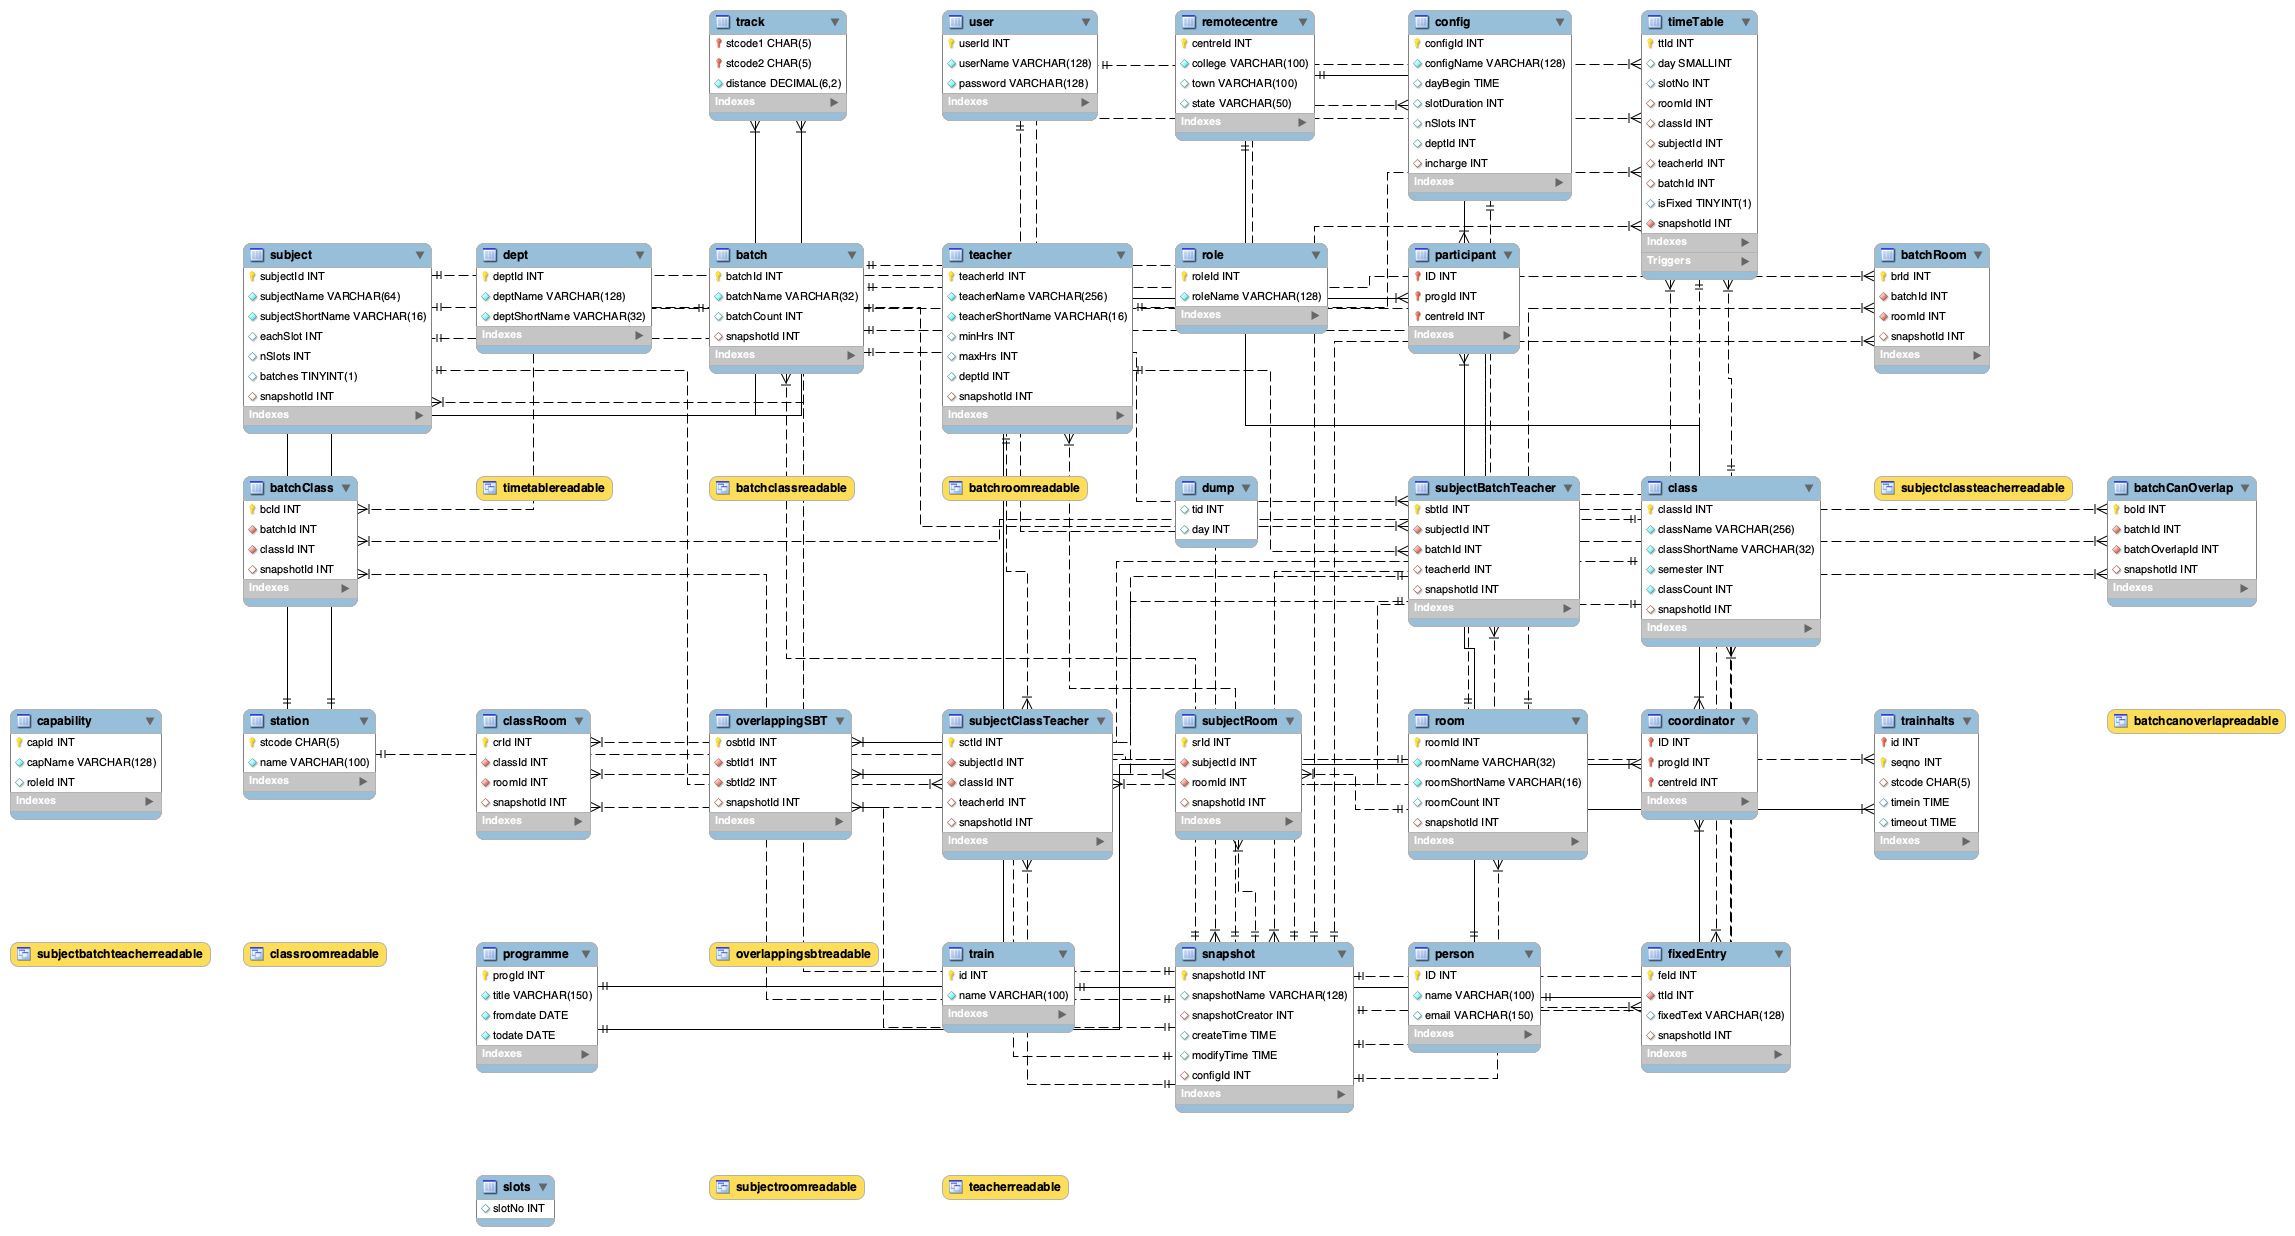
\includegraphics[width=0.62\textwidth]{figures/taasika-schema.png}
\caption{Schema of the Taasika scheduling database, the source of the pipeline.}
\label{fig:taasikaschema}
\end{figure}

A deliberate design decision was to parse the SQL dump textually rather than restore it into a
MySQL server. The loader (\texttt{scripts/taasika\_loader.py}) reads the dump and exposes each table
as a list of Python dictionaries filtered to a chosen snapshot. The pipeline therefore has no
database dependency, runs on any machine with Python, and treats the dump as an immutable input.

\subsection{Pipeline structure}

Figure~\ref{fig:pipeline} shows the complete path from the SQL dump to a scored timetable. Eight
generator modules run in dependency order, three validators check the result, and an archive step
produces the ZIP file that UniTime's Data Exchange page accepts.

\begin{figure}[H]
\centering
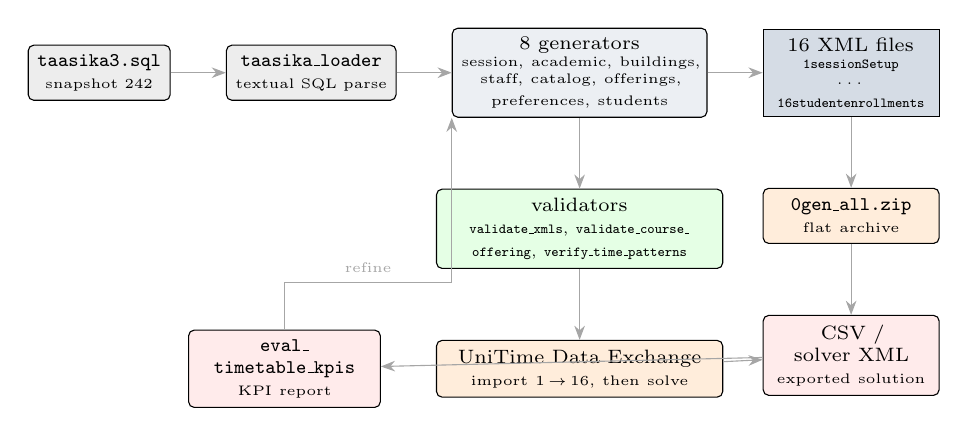
\begin{tikzpicture}[
  node distance=5mm and 7mm,
  src/.style={draw,rounded corners=2pt,fill=gray!14,align=center,font=\scriptsize,minimum height=7mm},
  gen/.style={draw,rounded corners=2pt,fill=coepblue!8,align=center,font=\scriptsize,minimum height=7mm},
  xml/.style={draw,fill=coepblue!18,align=center,font=\scriptsize,minimum height=7mm},
  val/.style={draw,rounded corners=2pt,fill=green!10,align=center,font=\scriptsize,minimum height=7mm},
  ut/.style={draw,rounded corners=2pt,fill=orange!14,align=center,font=\scriptsize,minimum height=7mm},
  ev/.style={draw,rounded corners=2pt,fill=red!8,align=center,font=\scriptsize,minimum height=7mm},
  ar/.style={-{Stealth[length=1.8mm]},gray!70}
]
\node[src] (sql) {\texttt{taasika3.sql}\\{\tiny snapshot 242}};
\node[src, right=of sql] (load) {\texttt{taasika\_loader}\\{\tiny textual SQL parse}};
\node[gen, right=of load, text width=30mm] (gens) {8 generators\\{\tiny session, academic, buildings,\\staff, catalog, offerings,\\preferences, students}};
\node[xml, right=of gens, text width=20mm] (xmls) {16 XML files\\{\tiny \texttt{1sessionSetup}\\$\dots$\\\texttt{16studentenrollments}}};

\node[val, below=9mm of gens, text width=34mm] (vals) {validators\\{\tiny \texttt{validate\_xmls},
\texttt{validate\_course\_offering}, \texttt{verify\_time\_patterns}}};
\node[ut, below=9mm of xmls, text width=20mm] (zip) {\texttt{0gen\_all.zip}\\{\tiny flat archive}};

\node[ut, below=9mm of vals, text width=34mm] (ut) {UniTime Data Exchange\\{\tiny import 1\,$\rightarrow$\,16, then solve}};
\node[ev, below=9mm of zip, text width=20mm] (out) {CSV / solver XML\\{\tiny exported solution}};
\node[ev, left=of ut, text width=22mm] (kpi) {\texttt{eval\_timetable\_kpis}\\{\tiny KPI report}};

\draw[ar] (sql) -- (load);
\draw[ar] (load) -- (gens);
\draw[ar] (gens) -- (xmls);
\draw[ar] (xmls) -- (zip);
\draw[ar] (gens) -- (vals);
\draw[ar] (vals) -- (ut);
\draw[ar] (zip) -- (out);
\draw[ar] (ut) -- (out);
\draw[ar] (out) -- (kpi);
\draw[ar] (kpi.north) -- ++(0,6mm) -| node[pos=0.25,above,font=\tiny]{refine} (gens.south west);
\end{tikzpicture}
\caption{The taasika-v3 pipeline. Data flows left to right and top to bottom; the dashed return
path is the refinement loop described in Section~\ref{sec:evaluation}.}
\label{fig:pipeline}
\end{figure}

\subsection{The sixteen imports and why their order matters}

UniTime's Data Exchange interface accepts one document per entity type, and each document
references entities created by an earlier one. The files are numbered so that the import order is
unambiguous; Appendix~\ref{app:imports} lists all sixteen with the dependency that fixes each
position. Three positions are worth highlighting:

\begin{itemize}
  \item \textbf{File 1 is absolute.} \texttt{1sessionSetup.xml} creates the academic session,
    departments, subject areas, solver groups, date patterns and time patterns. Nothing can be
    imported before it exists.
  \item \textbf{File 13 is not optional.} \texttt{13preferences.xml} attaches a time pattern and a
    date pattern to every scheduling subpart. Without it UniTime treats the classes as
    ``arrange hours'' and does not load them into the solver at all, which presents as a solver
    reporting a handful of variables instead of several hundred.
  \item \textbf{Files 14--16 must follow 12.} Student records, course requests and section
    enrolments all reference classes by the identifiers established in
    \texttt{12courseOffering.xml}.
\end{itemize}

Two operational details cost significant time and are recorded here because neither is obvious from
the documentation. First, the term identifier used by the Data Exchange API is the academic term
followed by the year with no separator---\texttt{Spr122026}, not \texttt{2026Spr12}. Second, the
archive must contain the sixteen documents at its \emph{root}; building it with
\texttt{zip -r 0gen\_all.zip 0gen\_all} nests them inside a directory and the import silently fails
to find them. Both the pipeline's own archive step and the standalone
\texttt{scripts/zip\_0gen\_all.py} write entries with a flattened name for this reason.

\subsection{Design decisions}

The Taasika dump does not carry every field UniTime requires, and several structural differences
between the two models had to be resolved by rule rather than by lookup. Table~\ref{tab:decisions}
records the decisions actually implemented in the generators.

\begin{table}[H]
\centering
\caption{Mapping decisions implemented in the generator scripts.}
\label{tab:decisions}
\footnotesize
\begin{tabular}{@{}L{3.5cm}L{11.4cm}@{}}
\toprule
\textbf{Decision} & \textbf{Rule implemented} \\
\midrule
Lecture\,+\,laboratory merging &
  A laboratory or tutorial subject is merged into its lecture partner when its short name is the
  lecture's short name plus one of \texttt{-Lab}, \texttt{Lab}, \texttt{-Tut}, \texttt{Tut} or
  \texttt{-Tutorial}. The merged course becomes one offering with one configuration and two
  subparts, so joint lectures and parallel batches live under a single course. \\
Course credits &
  The Indian engineering convention: one credit per lecture hour and half a credit per laboratory
  hour, so a three-hour lecture paired with a two-hour laboratory yields four credits. Unpaired
  subjects use the lecture-only or laboratory-only half of the same formula, with a floor of one. \\
Class identifiers &
  Human-readable and stable: \texttt{"<area> <courseNbr> <type> <suffix>"}, for example
  \texttt{CS 110 Lab 3}. These identifiers are what files 15 and 16 reference. \\
Building inference &
  Taasika stores room names but not buildings. A heuristic on the room name and short name assigns
  each room to one of six inferred buildings; unavailable laboratories are collected into their own
  pool so that their use remains visible in the KPI report. \\
Instructor position &
  Derived from each teacher's \texttt{minHrs}/\texttt{maxHrs} envelope: at most 6 hours maps to
  professor, at most 12 to associate professor, otherwise assistant professor, with
  $(0,0)$ mapped to adjunct and $(0,24)$ to visitor. \\
Times left unsolved &
  No class carries a \texttt{<time>} element. The existing Taasika timetable rows are deliberately
  not imported as preferences, because the object of the exercise is for UniTime to solve the
  timetable rather than to reproduce the manual one. \\
Rooms as preferences &
  Room associations from Taasika are emitted as preferences, not as pre-assignments, leaving the
  solver free to choose. \\
Student simulation &
  The institution's MIS data was not available, so students are generated from confirmed headcounts
  (Section~\ref{sec:datasets}) with synthetic identifiers of the form \texttt{61yy03aaa}. \\
\bottomrule
\end{tabular}
\end{table}

\subsection{Entry point and validation}

The whole pipeline is driven by one command, which selects the SQL dump and snapshot, runs the
eight generators in order, runs the three validators, and writes the archive only if all three
pass:

\begin{lstlisting}[style=plainlst,language=bash,caption={Regenerating the complete dataset.}]
python scripts/gen_all.py --term Spr12 --sql taasika-db/taasika3.sql --snapshot 242
\end{lstlisting}

The validators check three different properties. \texttt{validate\_xmls.py} confirms that every
generated document is well-formed XML. \texttt{validate\_course\_offering.py} checks the structural
invariants of file 12---that every class belongs to a subpart, every subpart to a configuration,
and every configuration to an offering---before UniTime is given the chance to reject it.
\texttt{verify\_time\_patterns.py} re-derives each subject's weekly minutes from the Taasika
snapshot and confirms that the time pattern emitted in file 13 matches, which catches the class of
error where a course silently becomes unschedulable because its duration has no matching pattern.

A separate script, \texttt{scripts/zip\_0gen\_all.py}, re-targets an existing dataset to a new term
and rebuilds the archive without regenerating from SQL. This exists because a fresh UniTime
academic session is often the fastest way to recover from a bad import, and creating one requires
only that the term attribute change.

\section{Institution-Specific Constraints}
\label{sec:constraints}

\subsection{Inherited constraint mapping}

The Semester~VI phase identified the institution's scheduling rules and established that each is
expressible within UniTime's constraint model. Table~\ref{tab:inherited} reproduces that mapping,
which remains valid and is the starting point for this section.

\begin{table}[H]
\centering
\caption{Constraint mapping established in Semester VI.}
\label{tab:inherited}
\footnotesize
\begin{tabular}{@{}L{5.0cm}L{9.9cm}@{}}
\toprule
\textbf{Constraint} & \textbf{Mechanism in UniTime} \\
\midrule
Distance between rooms & Distance check integrated into the room detail configuration. \\
Preferred labs and lectures & Subparts within an instructional offering, each with its own time pattern. \\
Evenly distributed working hours & Instructor preference settings; the solver favours consecutiveness. \\
Minimisation of schedule holes & The \texttt{StudentMinimizeScheduleHoles} optimisation criterion. \\
Consecutive lectures for a course & Distribution preferences favouring adjacent slots on the same day. \\
Maximum slots per course per day & Distribution preferences imposing a per-day limit. \\
Instructor load management & Distribution preferences limiting back-to-back classes. \\
Departmental cohort conflicts & Distribution preferences preventing overlap for a shared cohort. \\
Specialised laboratory allocation & Room groups encoding hardware and equipment requirements. \\
Common university hours & Reserved slots excluded from the time-pattern configuration. \\
\bottomrule
\end{tabular}
\end{table}

\subsection{From mapping to implementation}

A mapping records that a rule \emph{can} be expressed; it does not schedule anything. The work of
this phase was to generate the corresponding data for every class in the dataset, so that the rules
are reproduced automatically each time the pipeline runs rather than re-entered by hand after each
import. Table~\ref{tab:implemented} lists what is actually emitted, and where.

\begin{table}[H]
\centering
\caption{Constraints as implemented in the generated data.}
\label{tab:implemented}
\footnotesize
\begin{tabular}{@{}L{3.6cm}L{5.0cm}L{6.2cm}@{}}
\toprule
\textbf{Rule} & \textbf{Where it is produced} & \textbf{Form} \\
\midrule
Meeting patterns & \texttt{gen\_preferences.py} & a \texttt{<timePref>} naming one of the ten
  session time patterns, on every subpart and class \\
Date pattern & \texttt{gen\_preferences.py} & \texttt{Full Term} date preference at required level \\
Minor-degree block & \texttt{FIXED\_ENTRIES\_MAP} & required Monday/Tuesday 16:30--18:30 window \\
Open-elective block & \texttt{FIXED\_ENTRIES\_MAP} & required Monday/Tuesday 09:30--10:30 window \\
Protection of both blocks & \texttt{FIXED\_ENTRIES\_MAP} & prohibited windows on all other courses \\
Room preferences & \texttt{gen\_preferences.py} & \texttt{<roomPref>} lists derived from Taasika
  room associations, never pre-assignments \\
Specialised laboratories & \texttt{gen\_buildings.py} & building inference plus a separate pool for
  unavailable laboratories \\
Lunch breaks & \texttt{setup\_lunch\_breaks.py} & solver criteria, applied server-side \\
Division and batch structure & \texttt{gen\_academic.py}, \texttt{gen\_students.py} & 242 student
  groups; membership derived from enrolment \\
Weekend exclusion & \texttt{gen\_buildings.py} & room sharing marks weekends unavailable \\
Travel times & \texttt{gen\_buildings.py} & 5 minutes between buildings, 3 between the two CSE
  buildings \\
\bottomrule
\end{tabular}
\end{table}

\subsection{The modular time-block mechanism}

The institution reserves fixed windows in the week for course categories that are taught across
departments. Minor-degree courses meet on Monday and Tuesday evenings; open electives meet on
Monday and Tuesday mornings. These are not preferences but hard institutional commitments, and
they have a second half that is easy to overlook: if a window is reserved for one category, every
\emph{other} course must be kept out of it, or the reservation achieves nothing.

This was implemented as a small rule engine inside \texttt{gen\_preferences.py}. A rule table,
\texttt{FIXED\_ENTRIES\_MAP}, is consulted for every subpart; the first rule whose course pattern
matches, and whose exclusion pattern does not, becomes the active rule for that subpart.
Table~\ref{tab:fixedentries} lists the four rules currently in force.

\begin{table}[H]
\centering
\caption{The fixed time-block rules, in evaluation order.}
\label{tab:fixedentries}
\footnotesize
\begin{tabular}{@{}L{3.1cm}L{5.2cm}L{1.9cm}L{2.3cm}L{1.9cm}@{}}
\toprule
\textbf{Rule} & \textbf{Courses matched} & \textbf{Days} & \textbf{Window} & \textbf{Level} \\
\midrule
\texttt{MDM\_Required}        & \texttt{MDM*}                                   & Mon, Tue & 16:30--18:30 & Required \\
\texttt{OE\_Required}         & \texttt{OE*}                                    & Mon, Tue & 09:30--10:30 & Required \\
\texttt{Non\_MDM\_Prohibited} & everything except \texttt{MDM*}, \texttt{OE*}   & Mon, Tue & 16:30--18:30 & Prohibited \\
\texttt{SY\_Non\_OE\_Prohibited} & CO, CoI, DTL, DTL-Lab, Eco, OOPD, OOPD-Lab, TOC, TOC-Tut & Mon, Tue & 09:30--10:30 & Prohibited \\
\bottomrule
\end{tabular}
\end{table}

The two levels do different jobs. A required rule marks the one slot that matches the day set and
fits the window; a prohibited rule marks every candidate whose days and interval overlap the
window. The first pins a course into its block, the second clears the block for everyone else.
The second-year rule lists courses by name rather than by wildcard, because only that year's core
courses share the open-elective morning, and the list says so explicitly.

\subsection{Meeting patterns}

Each subpart's weekly contact minutes, read from the Taasika snapshot, determine its meeting
pattern. Lectures of 240 minutes per week become \texttt{2 x 120}, 180 become \texttt{3 x 60} and
120 become \texttt{2 x 60}; laboratories and recitations are single meetings, so 480 minutes becomes
\texttt{1 x 480 Project}, 180 becomes \texttt{1 x 180} and 120 becomes \texttt{1 x 120}. Anything
that does not match a declared pattern falls back to \texttt{Exact Time}, which
\texttt{verify\_time\_patterns.py} reports as an audit finding rather than passing silently. The
migration of lectures to the $2\times120$ pattern was a deliberate change made during this phase to
reflect how the department actually teaches.

\subsection{Lunch breaks}

The Semester~VI report proposed implementing a universal lunch break by excluding slots from the
assignable time patterns. That approach was rejected in implementation because it is too rigid: it
removes the same hour from every day for every class, whereas the institution requires only that
each student and each instructor have \emph{some} free hour within a window.

The implemented mechanism is a dynamic one-hour break between 11:30 and 15:30, applied to students
and to instructors, and installed as solver criteria by the Jython script
\texttt{scripts/unitime\_scripts/setup\_lunch\_breaks.py}, which is uploaded and run inside UniTime
through \textbf{Administration\,$\rightarrow$\,Utilities\,$\rightarrow$\,Scripts}. Rooms remain
available for the whole weekday. Because this is a soft criterion rather than a blocked slot, the
solver may violate it, and the evaluator of Section~\ref{sec:evaluation} therefore checks it
explicitly: the final solution leaves 63 students and one instructor without a qualifying break.

\subsection{Student groups and what they do not do}

The dataset declares 242 student groups, one for each Taasika class and each batch. Since the
pipeline's most recent change, every student is also made a member of the groups corresponding to
the classes they are enrolled in: the group code is taken from the class's schedule note, so a
student enrolled in the second-year division-one lecture is a member of \texttt{SY-Div1}, and a
student enrolled in a particular laboratory batch is a member of that batch's group.

Membership makes the cohort visible and is a prerequisite for a future group reservation. It does
not constrain the timetable. A student's groups affect course sectioning in one place only, a
distance computation used for students who are not yet enrolled, and the final sectioning pass does
not read them. With student switching off, adding the memberships changed no placement and no
conflict count. What actually pins a student to a section is file 16 together with the three
settings of Section~\ref{sec:setup}.

\subsection{Shared laboratory sessions}

A laboratory supervised by two instructors, in the same room at the same time for the same batch,
is represented through UniTime's support for multiple lead instructors on a single class. Courses
with several lecture or laboratory sections taught by different instructors are modelled as
separate classes under a common subpart, which is the same mechanism the pipeline uses to emit one
lecture class per Taasika class record and one laboratory class per batch record.

\section{Datasets Used}
\label{sec:datasets}

\subsection{The current dataset}

The working dataset is \texttt{unitime-out/0gen\_all}, a complete set of the sixteen Data Exchange
documents for a single academic session. Every file carries the term attribute \texttt{Spr12} and
the year \texttt{2026}, giving the Data Exchange term identifier \texttt{Spr122026}. The session
runs from 19 January 2026 to 22 May 2026, with classes ending on 30 April and the examination
period beginning on 4 May. The weekly grid is seven days of ten hourly slots from 08:30 to 18:30,
with the underlying solver resolution being five-minute slots.

Table~\ref{tab:dataset} gives the inventory, recomputed directly from the files rather than quoted
from documentation.

\begin{table}[H]
\centering
\caption{Inventory of \texttt{unitime-out/0gen\_all} (term \texttt{Spr122026}).}
\label{tab:dataset}
\footnotesize
\begin{tabular}{@{}rL{5.0cm}rL{6.6cm}@{}}
\toprule
\textbf{\#} & \textbf{File} & \textbf{Bytes} & \textbf{Contents} \\
\midrule
1  & \texttt{1sessionSetup.xml}            &  12{,}486 & session, departments, subject areas, date and time patterns \\
2  & \texttt{2academicArea.xml}            &     496 & 2 areas (B.Tech, M.Tech) \\
3  & \texttt{3academicClassification.xml}  &     786 & 5 year codes (FY, SY, TY, BT, MT) \\
4  & \texttt{4Major.xml}                   &   1{,}832 & 15 majors \\
5  & \texttt{5Minor.xml}                   &     374 & empty by design; Taasika models minors as majors \\
6  & \texttt{6studentGroup.xml}            &  25{,}485 & \textbf{242 groups} (43 classes + 199 batches) \\
7  & \texttt{7buildingRoomImport.xml}      &  21{,}604 & \textbf{6 buildings, 42 rooms} \\
8  & \texttt{8roomSharing.xml}             &   9{,}916 & 45 sharing blocks; weekends unavailable \\
9  & \texttt{9travelTimes.xml}             &   2{,}722 & 7 inter-building travel entries \\
10 & \texttt{10staff.xml}                  &  19{,}618 & \textbf{115 instructors} \\
11 & \texttt{11courseCatalog.xml}          &  44{,}081 & \textbf{158 courses} \\
12 & \texttt{12courseOffering.xml}         & 100{,}340 & \textbf{56 offerings, 84 subparts, 291 classes} \\
13 & \texttt{13preferences.xml}            &  95{,}146 & 362 preference blocks \\
14 & \texttt{14studentInfo.xml}            & 657{,}518 & \textbf{1{,}130 students}, 5{,}767 group references \\
15 & \texttt{15studentRequest.xml}         & 495{,}638 & course requests for 1{,}130 students \\
16 & \texttt{16studentenrollments.xml}     & 661{,}230 & \textbf{9{,}148 section enrolments} \\
\bottomrule
\end{tabular}
\end{table}

\subsection{Source snapshot}

Determining which Taasika snapshot produced this dataset required evidence rather than trust. Four
of the files carry the attribute \texttt{created="Generated from Taasika snapshot 240"}, but that
string is hard-coded in three of the generator scripts and is not updated when a different snapshot
is selected, so it cannot be used as provenance. The snapshot was therefore identified by counting.

\begin{table}[H]
\centering
\caption{Identifying the source snapshot by counting entities.}
\label{tab:snapshot}
\footnotesize
\begin{tabular}{@{}L{4.6cm}rrrl@{}}
\toprule
\textbf{Quantity} & \textbf{Snap 240} & \textbf{Snap 242} & \textbf{Snap 263} & \textbf{\texttt{0gen\_all}} \\
\midrule
Classes + batches = groups & $43{+}165={}$208 & $43{+}199={}$\textbf{242} & $32{+}128={}$160 & \textbf{242} \\
Teachers                   & 113 & \textbf{115} & 67 & \textbf{115} \\
Rooms                      & 49  & 49  & 29 & 42 (see below) \\
\bottomrule
\end{tabular}
\end{table}

The dataset was generated from snapshot \textbf{242}, named \texttt{published-v4-26jan26}, in
\texttt{taasika-db/taasika3.sql}. Snapshot 240 is the Semester~VI dataset and is what
\texttt{unitime-out/README.md} still documents; snapshot 263 is a later snapshot for the following
academic year that was integrated into the loader but is not the source of these files. The stale
provenance string is recorded as a known defect in Section~\ref{sec:limitations}.

The room count differs from the snapshot because the pipeline no longer emits the virtual
``Online'' building: 49 rooms in the snapshot less seven online rooms gives the 42 that are
imported. The six buildings are the Academic Complex (14 rooms), the Computer Engineering and IT
department (15), the ENTC Extension (5), the New CSE Building (2), the Bhau Institute (2), and a
pool of four laboratories marked unavailable, which is retained deliberately so that any use of
them remains visible in the evaluation report.

\subsection{Student population}

Institutional MIS data was not available, so the student body is simulated from headcounts
confirmed with the department and recorded in \texttt{scripts/intake.py}.
Table~\ref{tab:students} gives the composition. Identifiers follow the pattern \texttt{61yy03aaa},
where \texttt{yy} encodes the year of study. No real student data appears anywhere in the
repository or in this report.

\begin{table}[H]
\centering
\caption{Simulated student population of the current dataset.}
\label{tab:students}
\footnotesize
\begin{tabular}{@{}lrrrL{6.2cm}@{}}
\toprule
\textbf{Year} & \textbf{CSE} & \textbf{AI\,\&\,ML} & \textbf{Total} & \textbf{Structure} \\
\midrule
First year (FY)   & 300 & 100 & 400   & single cohort, reserved blocks \\
Second year (SY)  & 200 & 0   & 200   & two lecture divisions; direct second-year entrants join here \\
Third year (TY)   & 200 & 0   & 200   & two divisions, departmental electives \\
Final year (BT)   & 200 & 0   & 200   & two divisions, one departmental elective each \\
M.Tech (MT)       & \multicolumn{2}{c}{130} & 130 & specialisation streams \\
\midrule
\textbf{Total}    &     &     & \textbf{1{,}130} & all with enrolments \\
\bottomrule
\end{tabular}
\end{table}

Minor-degree and open-elective provision is modelled as room blocks rather than as enrolments,
because those courses are taught by other departments: 600 seats are reserved for minor-degree
teaching across the second, third and final years, and 200 for the second-year open elective.

Two known imperfections in the simulation are recorded rather than hidden. Two hundred first-year
students could not be placed in \texttt{CS PPS-FY Lec} because the declared section limits do not
cover the cohort, and two M.Tech students overflow the \texttt{PSEC2-EAI} laboratory. The section
filling routine assigns students to a preferred section up to its declared limit and then spills
into later sections of the same course and type, which is also why a small number of laboratory
batches contain students drawn from two different lecture divisions.

\subsection{Other instances used in the experiments}

Several earlier instances appear in Section~\ref{sec:experiments}, and their counts differ. The
term labels are \emph{not} different semesters: \texttt{Spr6}, \texttt{Spr10}, \texttt{Spr11} and
\texttt{Spr12} are successive UniTime academic sessions created for Spring 2026, each a clean
re-import of an evolving dataset. Table~\ref{tab:instances} lists them so that no figure in this
report appears without its denominator.

\begin{table}[H]
\centering
\caption{Instances referenced in this report.}
\label{tab:instances}
\footnotesize
\begin{tabular}{@{}L{4.4cm}lrrrL{4.0cm}@{}}
\toprule
\textbf{Instance} & \textbf{Session} & \textbf{Classes} & \textbf{Students} & \textbf{Rooms} & \textbf{Role} \\
\midrule
\texttt{rl/instances/spr2026.xml}        & Spr6  & 262 & 990   & 44 & solver export used for all headless experiments \\
\texttt{spr2026\_10m\_w5.xml}            & Spr6  & 262 & 990   & 44 & already conflict-free; bake-off instance \\
\texttt{spr2026\_10\_LE\_SS\_Enrolled}   & Spr10 & 290 & 1{,}130 & 41 & first pinned-enrolment run \\
\texttt{spr2026\_11\_all\_flags.csv}     & Spr11 & 291 & 1{,}130 & 42 & final solution, scored in Section~\ref{sec:experiments} \\
\texttt{unitime-out/0gen\_all}           & Spr12 & 291 & 1{,}130 & 42 & current input dataset \\
\bottomrule
\end{tabular}
\end{table}

The 990 figure recurring in the Spr6 rows is the number of students that the UniTime solver export
carried enrolments for, out of a simulated roll of 1{,}290 in the dataset of that period. The gap
is not attrition; it is the difference between the students the solver loaded and the students that
existed in the source files, and it is the origin of the conflict-rate reconciliation in
Section~\ref{sec:experiments}.

\section{Simulation, Testing and UniTime Debugging}
\label{sec:simulation}

Students had to be simulated because of the following reasons:

A timetable can be created without students (only classes, rooms, instructors, preferences are needed).
You cannot \emph{evaluate} it without them, though.
The most important metric the institute cares about is whether there are any overlapping classes in a student's weekly schedule, but that isn't meaningful until students are put into sections.

Because of the lack of data about students at the institute, we used simulated students.
The simulation is not random, it is deterministic.
It begins with the actual number of students in each year, partitions students into lecture groups, assigns students to lab groups within each lecture group, and generates course requests for all required courses and one elective course per group of students.
Finally, it adds each student to a particular lecture section and lab section, creating the 9{,}148 enrolment rows in file 16.

The filling of the sections and the consequences thereof.

Enrolments are assigned one section at a time.
Each student goes into their division's preferred section until it hits the limit in the offering file, then spills into later sections of the same course and type.
This is similar to what is typically observed in over-subscribed labs, and it leaves two clear imprints on the data.

First, some lab batches are mixed, with students from two different lecture divisions being in the same batch as one division's preferred batches filled first.
This is a combination of three final year lab batches.
Second, if the section size is too small for a cohort, additional students remain unplaced and are not dropped silently from the generator, but rather logged.
That's why 200 first-year students and two M.Overflow of tech lab in Section~\ref{sec:datasets}.

These are both effects of the \emph{input data} and not the solver.
They are tracked because they are a tie that binds two divisions together in an unusual way, which can cause conflict where it is not expected.

\subsection{Conflict types encountered}

During this stage, three types of student conflict emerged and we needed to distinguish each type before we could do anything about it:

\begin{itemize}
  \item True overlap of two classes that the student is truly enrolled in. These are the types of conflicts that the solver should delete, and all 40 remaining conflicts in the final solution are of this type.
  \item Artefacts of cross-division batches, where a clash only occurs as a result of a student being placed in another division's batch by section filling.
  \item Artefacts of measurement: where the number of students reported has changed due to changes in the student population, rather than the timetable. Section~\ref{sec:experiments} analyses these.
\end{itemize}

\subsection{UniTime debugging log}

A significant amount of time was lost searching for import and solver failures that did not provide any useful error message.
This is not documented in the UniTime docs, so each symptom is listed with its root cause and fix in Table~\ref{tab:debug}.

\begin{table}[H]
\centering
\caption{Import and solver failures that were observed, with their causes and resolutions.}
\label{tab:debug}
\footnotesize
\begin{tabular}{@{}L{4.0cm}L{5.4cm}L{5.4cm}@{}}
\toprule
\textbf{Symptom} & \textbf{Cause} & \textbf{Resolution} \\
\midrule
Every class reports \emph{``has no available room (class not loaded)''} although all rooms imported
  & Buildings, built by file 7, are global and not scoped to the session, so no session has buildings
    until it is told to pick them up
  & \textbf{Administration\,$\rightarrow$\,Academic Sessions\,$\rightarrow$\,Buildings\,$\rightarrow$\,Update Data}, then reload the solver \\
Solver loads a few variables rather than hundreds
  & If there is no time pattern on the subpart, UniTime treats the class as ``arrange hours'' and excludes
    it from the solver
  & Import \texttt{13preferences.xml}, and re-import it whenever offerings are reloaded \\
The imported archive is empty
  & Data Exchange reads the archive root; \texttt{zip -r} puts the documents in a directory
  & Flatten the name of the entries, as the archive scripts do now \\
Teachers are not attached to classes
  & The staff imported by file 10 are not yet in the session's instructor list
  & \textbf{Courses\,$\rightarrow$\,Input Data\,$\rightarrow$\,Instructors\,$\rightarrow$\,Manage Instructor List} \\
Solver reports \texttt{Student conflicts: 0} and exports an empty student block
  & \emph{Projected Student Course Demands} reads last-like demand and curriculum projections;
    where the session has neither, zero students load
  & Set \emph{Student Course Demands} to \emph{Enrolled Student Course Demands} and reload \\
Re-importing offerings deletes classes unexpectedly
  & \texttt{incremental="true"} will not delete unmatched offerings, but will delete unmatched
    classes within offerings in the file
  & Uncommit any saved solution first, and treat file 12 as authoritative for the offerings it mentions \\
The exported solver XML has no class or room names
  & By default, the solution export is anonymised
  & Set \texttt{unitime.solution.export.names=true} in
    \textbf{Administration\,$\rightarrow$\,Defaults\,$\rightarrow$\,Configuration} \\
Student group import fails with a Hibernate \texttt{TransientObjectException}
  & Combining two large groups into one transaction
  & Emit group membership in the student records of file 14, rather than as bulk group updates \\
\bottomrule
\end{tabular}
\end{table}

The tendency to assign pupils to their sections.

The most significant thing we've discovered is how UniTime deals with imported enrolments.
The database loader loads each \texttt{StudentClassEnrollment} row, and attaches the student to the class provided that the student has already been attached to that course offering, and that the student is permitted to be attached to that class.
The initial sectioning still continues after the sectioning, but it does not include students who are already in the class, and the loader will only log a warning if a student left their loaded class.
To summarize: UniTime respects imported enrolments, if you tell the solver to do so.

All three are required:

\begin{enumerate}
  \item Enrolments are read at all, with \emph{Student Course Demands} set to \emph{Enrolled Student Course Demands}.
  \item \texttt{General.SwitchStudents=false}, so the last sectioning pass does not move students between parallel sections to hide conflicts.
  \item \texttt{Global.LoadStudentEnrlsFromSolution=true}, so sections are loaded from the stored enrolments and not recomputed.
\end{enumerate}

With these enabled, the conflict count rises from an apparent zero to a real 40, exactly what we wanted to see: see Section~\ref{sec:experiments}.

\section{Evaluation Framework and Tools}
\label{sec:evaluation}

\subsection{Why an external evaluator was required}

The quality of its own solutions: percentage of variables assigned, room, time
A student conflict count, a preference satisfaction and a preference satisfaction. The data in these figures are based on the solver's
The thing under test, internal model. When the model loads no students, the student
conflict count equals 0---if the model re-sections students, then this count is also 0. Neither
The latter two are also false from the solver's perspective, and have no value to the institution.

A third party assessment was thus prepared. It takes a timetable and the \emph{input} XML as
Two different arguments and re-derives each quantity anew: which student is which.
of which class comes from the enrolment file, when each class meets comes from the solution, and the
two are connected together by the evaluator instead of by the solver. Failure to load students.
The evaluator never asks the solver any questions and cannot propagate into the score.

Two ways to represent a denominator, two modes.

The distinction is \texttt{scripts/eval\_timetable\_kpis.py} is run in one of two modes.
The one most crucial thing to know about each number in Section~\ref{sec:experiments}.

\begin{description}[leftmargin=1.6em,style=nextline]
  \item[CSV mode]   The scores are exported from the UniTime's solver screen or saved-timetables and represent a timetable in CSV mode.
  screen. A UniTime CSV will not have any student column in it, and the evaluator will add class times to an
  An XML file of enrolments in the dataset directory. The denominator is the number of students in that, therefore.
  file.
\item[XML mode] is an XML processing capability that directly processes a CPSolver solver-model XML. This type of file is self-contained:
The rooms, classes, constraints, as well as the current assignment \emph{and} the student block.
The denominator are the students that were actually loaded.
\end{description}

The two denominators are unequal when the solver loaded a sub-set of students that is less than the number of students in the data,
On the Spr6 instances this equated to 990:1,290 respectively. These rates appear to be mixed together and result in a similar rate.
contradictory but are simply measurements of different populations. The figures in this report are
Reported with the mode and the denominator which gave it.

\subsection{What is measured}

The evaluator performs 10 hard checks, three preference checks and a series of efficiency metrics;
Appendix~\ref{app:kpis} gives the definition of each. A further check, \texttt{room\_unavailable},
applies to XML mode only and is not one of the ten. The hard feasibility score is an
equal-weight average of the hard check pass rates, and the preference score an average of the
On a scale of 0 to 100, both preferences and preferences rates. The aggregate alone would not be a good indicator, therefore the
evaluator always prints up to eight example failures per check and the component rates.
What makes the first-year conflict cluster of Section~\ref{sec:experiments} so simple is that the situations in both cases are just as simple.The first-year conflict cluster of Section~\ref{sec:experiments} is easy to understand because both situations are easy to understand.
localise.

The conflict rule and its cross validation

When two classes share the same day, and their slot intervals overlap, then the two classes conflict for a student.
When both endpoints have date patterns and---excluding endpoints touching each other---they have at least one active.
week. The same rule is used for the Python evaluator and the Java conflict as well.
oracle written for the learning layer.

That duplication proved to be helpful. Scoring your solution file
The student is reported by the java oracle in (\path{rl/runs/sweep/w5/spr2026/B1/seed1/solution.xml}).
If the violation rate is $0.026262626$ and the Python evaluator throws back $0.026263$ then there are 26 conflicted.
students out of 990. The agreement is accurate to the accuracy of printing. Two implementations written
on the other hand, to the same specification, in other languages, with other data structures, arriving at
the same count represents the most compelling evidence throughout the conflict that the definition of conflict adopted.
this report is properly put into effect.

The java oracle is unit-tested by itself, for a complete recompute over 200 batches of random numbers.
checks incremental update path, not its definition, as in moves.

\subsection{Supporting tools}

\begin{itemize}
  \item \texttt{convert\_xml\_to\_csv.py} takes a solver XML and puts it into the flat CSV form, so that a
    A headless solution can be scored with the same CSV path that can be used for a UniTime export.
  \item \texttt{relabel\_timetable\_csv.py} will rewrite the course column from the numeric value of UniTime to its name.
    Convert course numbers to short codes in Taasika: \texttt{CS 102} to \texttt{CS CN}. Without
    this a timetable is not legible to staff checking it.
  \item \texttt{generate\_timetable\_html.py} renders a weekly grid to HTML to be visually inspected, and
    Which is how structural errors like an entire year for one afternoon came to light.
    before any metric was computed.
  \item \texttt{verify\_time\_patterns.py} is a tool to verify the patterns that have been generated against the source durations.
  The program \texttt{validate\_xmls.py} 
  \item \texttt{validate\_course\_offering.py} validate for well-formedness
    and providing structure prior to import.
\end{itemize}

\subsection{The refinement loop}

These tools are used as a cycle, NOT as a one-shot check. Figure~\ref{fig:loop} shows the
The process that the phase adapted to was: create the data set, import and solve, export, evaluate,
Diagnose the worst failing check, change the generator or the configuration and re-generate. The
important property is that the only manual step is the diagnosis; everything else is scripted, so a
The changing of a constraint rule can be performed without hand editing to a scored timetable.

\begin{figure}[H]
\centering
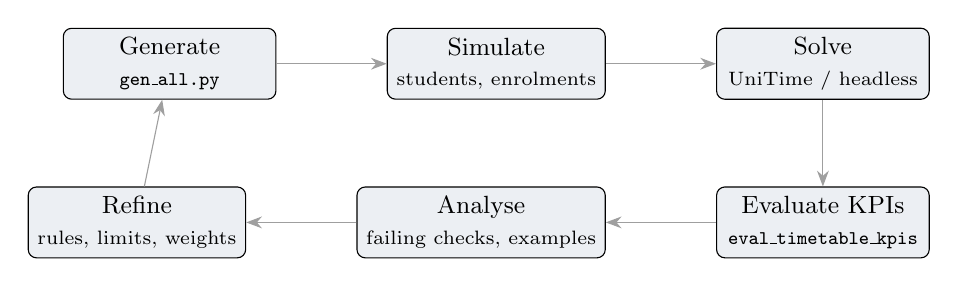
\begin{tikzpicture}[
  node distance=14mm,
  stg/.style={draw,rounded corners=3pt,align=center,font=\small,minimum width=27mm,minimum height=9mm,fill=coepblue!8},
  ar/.style={-{Stealth[length=2mm]},gray!75}
]
\node[stg] (gen) {Generate\\{\scriptsize \texttt{gen\_all.py}}};
\node[stg, right=of gen] (sim) {Simulate\\{\scriptsize students, enrolments}};
\node[stg, right=of sim] (solve) {Solve\\{\scriptsize UniTime / headless}};
\node[stg, below=11mm of solve] (eval) {Evaluate KPIs\\{\scriptsize \texttt{eval\_timetable\_kpis}}};
\node[stg, left=of eval] (analyse) {Analyse\\{\scriptsize failing checks, examples}};
\node[stg, left=of analyse] (refine) {Refine\\{\scriptsize rules, limits, weights}};

\draw[ar] (gen) -- (sim);
\draw[ar] (sim) -- (solve);
\draw[ar] (solve) -- (eval);
\draw[ar] (eval) -- (analyse);
\draw[ar] (analyse) -- (refine);
\draw[ar] (refine) -- (gen);
\end{tikzpicture}
\caption{ The iterative way of work during the phase. The only manual step is the \emph{Analyse} step;
All other transitions are scripted commands.}
\label{fig:loop}
\end{figure}

\subsection{Known limitations of the evaluator}

Two limitations are recorded so that its output is not over-read.

The \textbf{instructor identity check} is used to compare the instructor specified in the solution with the
The instructor expects from the Taasika data, and he gets 0\,\%. This is a
The following error message may come from name-format artefact, not a scheduling failure: UniTime is configured to export names in
The check will match ``Joshi, A'' against ``Amit Joshi'', and won't find a match to it.
any class. The basic task is right. The check must be normalised prior to its
output means anything.

A separate script can be found, \texttt{sectioning\_slot\_conflicts.py}, which keys on an exact
The string is \texttt{day start-end} and so it only recognizes time periods as a whole, not partial.
overlaps entirely. It does not report any conflicts when there are none, as well as a conflict for the one where there is.
This report does not include a figure.

\section{Experiments and Results}
\label{sec:experiments}

This section reports five experiments. The first three concern how student conflicts are measured
and whether the solver's objective can be tuned to reduce them; the fourth shows why several
apparently excellent results are not results at all; the fifth is the outcome of the phase.

\subsection{Solver checker versus KPI evaluator}

The first measurement to reconcile was a pair of figures that appeared to contradict each other on
the same term.

\begin{table}[H]
\centering
\caption{Two conflict rates for the Spr6 instance, and why they differ.}
\label{tab:reconcile}
\footnotesize
\begin{tabular}{@{}L{3.2cm}L{5.6cm}L{5.6cm}@{}}
\toprule
 & \textbf{Solver checker (Java)} & \textbf{KPI evaluator (CSV mode)} \\
\midrule
Value          & 526 of 990 conflicted, $C = 0.5313$ & 587 of 1{,}290 conflicted (45.5\,\%) \\
Instance       & \texttt{rl/instances/spr2026.xml} & \texttt{COEPSpr62026\_v2.csv} \\
Denominator    & students the solver loaded (990)  & all students in the enrolment file (1{,}290) \\
Membership     & the student block inside the solver file & re-derived by joining the CSV to file 16 \\
\bottomrule
\end{tabular}
\end{table}

The two are not inconsistent; they measure different populations of a different artefact. The
solver export carried enrolments for 990 of the 1{,}290 simulated students, and the CSV scored a
different exported solution. As Section~\ref{sec:evaluation} established, the two implementations
agree exactly when pointed at the same file. The lesson taken forward was procedural: every
conflict figure in this report is stated with its instance and its denominator, and no two figures
are compared unless both match.

\subsection{Tuning the student-conflict weight in UniTime}

CPSolver prices each student clash through \texttt{StudentConflictWeight}, and
\texttt{HardStudentConflictWeight} adds a further charge when the student has no alternative
section to move to. Raising the first should buy fewer conflicts at the cost of other soft
criteria. Two runs were made in the UniTime interface and exported as CSV.

\begin{table}[H]
\centering
\caption{Conflict weight raised in the UniTime solver, scored in CSV mode against the then-current
dataset (1{,}290 students, 262 classes).}
\label{tab:weightcsv}
\footnotesize
\begin{tabular}{@{}lrrrr@{}}
\toprule
\textbf{Weight} & \textbf{Students conflicted} & \textbf{Pairs} & \textbf{Hard feasibility} & \textbf{Preference score} \\
\midrule
5  & 676 of 1{,}290 & 1{,}076 & 90.97 & 25.00 \\
20 & 894 of 1{,}290 & 2{,}126 & 88.96 & 24.19 \\
\bottomrule
\end{tabular}
\end{table}

Read naively this says that raising the weight makes the timetable worse, which would be a strange
property for an optimiser. The correct reading is that this is not a controlled experiment. The
CSV join re-derives student membership from an enrolment file that the solver did not necessarily
use, the two runs started from different states, and the instance itself was changing during this
period. The experiment's real value was in motivating the controlled version that follows. The
figure of 676 at weight 5 supersedes an earlier figure of 614 quoted in the project's presentation
material, which no committed artefact reproduces.

\subsection{A controlled weight sweep}

To tune the weight properly the instance must be held fixed and the only variable must be the
weight. This was done headlessly, outside the UniTime server, using the project's own solver
runner. The instance was \texttt{rl/instances/spr2026.xml} (262 classes, 990 students, loaded with
an initial conflict rate of $C = 0.5313$); each configuration was run for 900 seconds of
wall-clock time with three random seeds; the reference arm B0 used the stock weight of 0.2.

\begin{figure}[H]
\centering
\begin{tikzpicture}
\begin{axis}[
  width=0.78\textwidth, height=6.2cm,
  xmode=log, log basis x=10,
  xlabel={\small \texttt{Comparator.StudentConflictWeight}},
  ylabel={\small student violation rate $C$},
  xtick={0.2,0.5,1,2,5,10}, xticklabels={0.2,0.5,1,2,5,10},
  ymin=-0.004, ymax=0.085,
  grid=major, grid style={gray!22},
  legend style={font=\scriptsize,at={(0.98,0.97)},anchor=north east,draw=gray!40},
  tick label style={font=\scriptsize}, label style={font=\small},
]
\addplot[only marks,mark=o,mark size=1.7pt,gray!65] table[x=weight,y=C] {data/sweep_points.dat};
\addlegendentry{individual seeds}
\addplot[coepblue,very thick,mark=*,mark size=2.2pt] table[x=weight,y=C] {data/sweep_median.dat};
\addlegendentry{median of 3 seeds}
\addplot[red!70!black,dashed,very thick,domain=0.18:11,samples=2] {0.04141};
\addlegendentry{B0 reference ($C=0.0414$)}
\end{axis}
\end{tikzpicture}
\caption{Student violation rate against the student-conflict weight, on a fixed instance with a
900-second budget and three seeds per weight. Every weight at or above 0.5 improves on the stock
B0 configuration, and seed-to-seed variance is comparable to the effect size.}
\label{fig:sweep}
\end{figure}

\begin{table}[H]
\centering
\caption{Weight sweep, median over three seeds (recorded in \texttt{rl/runs/sweep/summary.md}).}
\label{tab:sweep}
\footnotesize
\begin{tabular}{@{}lrrrr@{}}
\toprule
\textbf{Arm} & \textbf{Weight} & \textbf{$C$ (median)} & \textbf{Assigned} & \textbf{Soft penalty} \\
\midrule
B0 & 0.2  & 0.0414 & 1.00 & 60 \\
B1 & 0.2  & 0.0343 & 1.00 & 62 \\
B1 & 0.5  & 0.0192 & 1.00 & 66 \\
B1 & 1    & 0.0263 & 1.00 & 67 \\
B1 & 2    & 0.0030 & 1.00 & 65 \\
B1 & 5    & 0.0000 & 1.00 & 69 \\
B1 & 10   & 0.0040 & 1.00 & 64 \\
\bottomrule
\end{tabular}
\end{table}

Two observations follow. First, the solver starts from $C = 0.5313$ and every configuration drives
it below 0.06 within the budget while keeping all 262 classes assigned, so the overwhelming
majority of the reduction comes from the search itself rather than from the weight. Second, the
weight does matter at the margin: the best setting reduces the residual rate by roughly an order of
magnitude relative to the stock value.

One caveat must be attached to the weight-5 row. Recomputing the medians from the per-seed metric
files currently on disk reproduces every row of Table~\ref{tab:sweep} except that one, for which
the stored files give a median of 0.0263 and make weight 2 ($C = 0.0030$) the minimum instead. The
discrepancy is confined to a single seed whose run appears to have been repeated after the summary
was written. The choice between the two readings does not affect any conclusion: measured against
B0's 0.0414, the best weight achieves a relative reduction of either 1.000 or 0.927, and both
clear the 25\,\% threshold that had been fixed in advance. The honest statement is that weight
tuning alone reduces the residual conflict rate by well over 25\,\%, not that it reaches exactly
zero.

\subsection{Why several ``zero conflict'' results are not results}

Four artefacts in the repository report zero student conflicts. None of them represents a better
timetable, and Table~\ref{tab:zeros} gives the mechanism in each case.

\begin{table}[H]
\centering
\caption{Zero-conflict results and their actual causes.}
\label{tab:zeros}
\footnotesize
\begin{tabular}{@{}L{4.6cm}L{3.0cm}L{6.8cm}@{}}
\toprule
\textbf{Artefact} & \textbf{Reported} & \textbf{Mechanism} \\
\midrule
\texttt{spr2026\_mihir.kpi.json}, \texttt{spr2026\_10m\_w5.kpi.json}
  & 0 of 990
  & Student switching and initial sectioning moved students between parallel laboratory batches
    until the overlaps vanished. The placements did not change; the cohort structure did. \\
\texttt{rl/runs/bakeoff-spr2026\_10m\_w5} (3 arms $\times$ 10 seeds, 900\,s)
  & 0 for all arms
  & The instance was \emph{already} conflict-free when loaded: the initial violation rate recorded
    in every metrics file is 0.0. A 900-second run that begins and ends at zero measures nothing
    about conflict reduction. \\
\texttt{spr2026\_10\_LE\_90m\_w5.kpi.json}
  & 0 of 0
  & No students were loaded at all. The rate is zero over an empty denominator. \\
\texttt{kpi\_report\_MacMini\_v1.json}
  & 0 of 2{,}130
  & A different and earlier instance with only 254 classes, and two instructor conflicts. \\
\bottomrule
\end{tabular}
\end{table}

The first row is the mechanism that mattered. UniTime's final sectioning pass is permitted, by
default, to move a student from one laboratory batch to another in order to resolve a clash. For a
university that assigns batches administratively this is not a solution but a corruption of the
input, and it makes the reported metric unfalsifiable: any timetable can be made conflict-free if
the students are allowed to move. The remedy is the three settings of Section~\ref{sec:setup}, and
applying them is what produced the final experiment.

\subsection{The final solution under pinned enrolments}

With \emph{Enrolled Student Course Demands} selected, \texttt{General.SwitchStudents} set to
\texttt{false} and \texttt{Global.LoadStudentEnrlsFromSolution} set to \texttt{true}, the solver
can no longer move students, and the conflict count becomes a property of the timetable alone. The
exported solution \texttt{spr2026\_11\_all\_flags.csv} was scored against the current dataset:

\begin{lstlisting}[style=plainlst,language=bash]
python scripts/eval_timetable_kpis.py \
    --csv unitime-out/spr2026_11_all_flags.csv \
    --data-dir unitime-out/0gen_all
\end{lstlisting}

\begin{figure}[H]
\centering
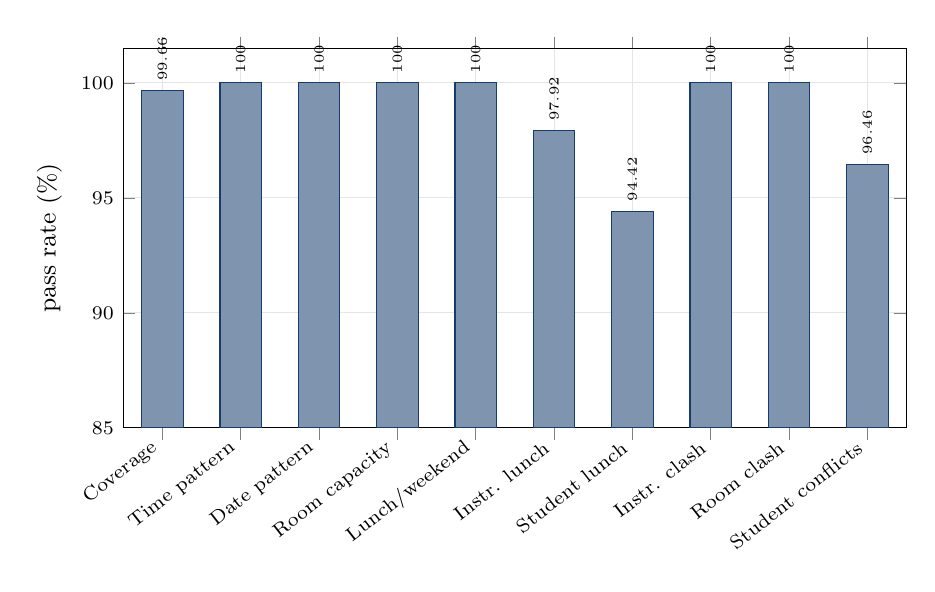
\begin{tikzpicture}
\begin{axis}[
  width=0.95\textwidth, height=6.4cm,
  ybar, bar width=15pt,
  ymin=85, ymax=101.5,
  ylabel={\small pass rate (\%)},
  symbolic x coords={Coverage,Time pattern,Date pattern,Room capacity,Lunch/weekend,Instr. lunch,Student lunch,Instr. clash,Room clash,Student conflicts},
  xtick=data,
  x tick label style={rotate=38,anchor=east,font=\scriptsize},
  tick label style={font=\scriptsize}, label style={font=\small},
  nodes near coords, every node near coord/.append style={font=\tiny,rotate=90,anchor=west},
  grid=major, grid style={gray!20},
  enlarge x limits=0.055,
]
\addplot[fill=coepblue!55,draw=coepblue] coordinates {
 (Coverage,99.66) (Time pattern,100) (Date pattern,100) (Room capacity,100)
 (Lunch/weekend,100) (Instr. lunch,97.92) (Student lunch,94.42)
 (Instr. clash,100) (Room clash,100) (Student conflicts,96.46)};
\end{axis}
\end{tikzpicture}
\caption{Hard-check pass rates of the final solution (term Spr11 solution scored against the
Spr12 dataset). The vertical axis starts at 85\,\% to make the three non-perfect checks legible.}
\label{fig:hardchecks}
\end{figure}

\begin{table}[H]
\centering
\caption{Full evaluation of the final solution: 291 classes, 1{,}130 students, 42 rooms,
115 staff.}
\label{tab:final}
\footnotesize
\begin{tabular}{@{}L{6.6cm}L{4.0cm}r@{}}
\toprule
\textbf{Metric} & \textbf{Value} & \textbf{Rate} \\
\midrule
Classes in offerings / in solution    & 291 / 291        & --- \\
Coverage                              & 290 of 291 assigned & 99.66\,\% \\
Hard feasibility score                & \textbf{98.85} / 100 & --- \\
Hard checks / failures                & 4{,}341 / 105    & --- \\
Time-pattern fidelity                 & 290 of 290       & 100\,\% \\
Date pattern                          & 290 of 290       & 100\,\% \\
Room capacity                         & 290 of 290       & 100\,\% \\
Lunch/weekend slot compliance         & 290 of 290       & 100\,\% \\
Instructor double-booking             & 0 conflicts      & 100\,\% \\
Room double-booking                   & 0 conflicts      & 100\,\% \\
\textbf{Student conflicts}            & \textbf{40 of 1{,}130 students, 40 pairs} & \textbf{96.46\,\%} \\
Student lunch breaks                  & 63 violations    & 94.42\,\% \\
Instructor lunch breaks               & 1 violation      & 97.92\,\% \\
Travel-time violations                & 0                & --- \\
Back-to-back density                  & 31.96\,\%        & --- \\
Unavailable/online room usage         & 17 of 291        & 5.84\,\% \\
Preference score                      & 6.29 / 100       & --- \\
\quad room preference                 & 35 of 278        & 12.59\,\% \\
\quad instructor identity             & 0 of 289 (artefact) & 0\,\% \\
\bottomrule
\end{tabular}
\end{table}

\paragraph{Interpretation.} The timetable is hard-feasible in every respect that the institution
treats as non-negotiable: no room is double-booked, no instructor is double-booked, every class
respects its meeting pattern and its room capacity, and 290 of 291 classes are placed. The
remaining student conflicts are a small and highly localised set. All 40 are first-year students,
and all 40 arise from the same pair of courses: a first-year programming laboratory overlapping the
first-year reserved lecture block, in four specific lab/lecture combinations---laboratory 1 against
reserved lecture 3 on Tuesday, laboratory 2 against reserved lecture 3 on Friday, laboratory 7
against reserved lecture 2 on Wednesday, and laboratory 9 against reserved lecture 1 or 2 on
Friday. Because the conflicts are concentrated in four placements rather than spread across the
cohort, they are addressable either by re-timing those four laboratories or by adding explicit
different-time distribution constraints between the laboratory and the reserved block.

Two results should not be over-read. The room preference rate of 12.59\,\% is genuinely poor and is
the clearest remaining optimisation target; it reflects that room preferences were generated
permissively from Taasika associations and that the solver traded them away cheaply. The
instructor identity rate of 0\,\% is not a result at all, but the name-format artefact described in
Section~\ref{sec:evaluation}.

\subsection{Cross-run comparison}

Table~\ref{tab:crossrun} collects every evaluated artefact so that no figure in this report
circulates without its context. The progression from the top group to the bottom row is the
substance of the phase: the apparent zeros disappear as the measurement is tightened, and what
remains is a small, real, diagnosable number.

\begin{table}[H]
\centering
\caption{All evaluated runs. CSV mode joins a timetable to an enrolment file; XML mode scores the
student block inside a solver file.}
\label{tab:crossrun}
\footnotesize
\begin{tabular}{@{}L{4.9cm}llrrr@{}}
\toprule
\textbf{Artefact} & \textbf{Mode} & \textbf{Instance} & \textbf{Classes} & \textbf{Conflicted} & \textbf{Hard feas.} \\
\midrule
\texttt{spr2026.kpi.json}               & XML & Spr6  & 262 & 526 / 990   & 92.15 \\
\texttt{kpi\_report.json}               & CSV & Spr6  & 260 & 587 / 1{,}290 & 94.98 \\
\texttt{kpi\_report\_2785.json}         & CSV & Spr6  & 262 & 507 / 1{,}290 & 92.66 \\
\texttt{kpi\_weight5\_report.json}      & CSV & Spr6  & 262 & 676 / 1{,}290 & 90.97 \\
\texttt{kpi\_weight20\_report.json}     & CSV & Spr6  & 262 & 894 / 1{,}290 & 88.96 \\
\texttt{solution.kpi.json} (sweep, $w{=}5$) & XML & Spr6 & 262 & 26 / 990 & 97.42 \\
\texttt{spr2026\_mihir.kpi.json}        & XML & Spr6  & 262 & 0 / 990 \textsuperscript{a} & 97.67 \\
\texttt{spr2026\_10m\_w5.kpi.json}      & XML & Spr6  & 262 & 0 / 990 \textsuperscript{a} & 98.26 \\
\texttt{spr2026\_10\_LE\_90m\_w5}       & XML & Spr10 & 290 & 0 / 0 \textsuperscript{b}   & 97.55 \\
\texttt{spr2026\_10\_LE\_SS\_Enrolled}  & XML & Spr10 & 290 & 32 / 1{,}130 & 97.77 \\
\textbf{\texttt{spr2026\_11\_all\_flags.csv}} & CSV & Spr11/12 & 291 & \textbf{40 / 1{,}130} & \textbf{98.85} \\
\bottomrule
\multicolumn{6}{@{}l@{}}{\footnotesize \textsuperscript{a} students re-sectioned;
  \textsuperscript{b} no students loaded. Neither is a conflict-reduction result.}
\end{tabular}
\end{table}

\section{Reinforcement-Learning Layer}
\label{sec:rl}

\subsection{Research question and hypothesis}

The weight sweep of Section~\ref{sec:experiments} tunes a single scalar. A more ambitious question
is whether the \emph{choice of search move} can be learned. At each step CPSolver's neighbourhood
selector picks a kind of move---change a time, change a room, swap two classes, ask for a
suggestion---according to fixed probabilities. The hypothesis of this part of the project was that
a policy conditioned on the state of the search could choose better than those fixed probabilities,
and thereby reach a lower student-conflict rate within the same budget.

A success criterion was fixed in advance: a learned policy would be considered to have succeeded if
it reduced the student violation rate by at least 25\,\% relative to a tuned baseline, at equal
wall-clock budget, on a held-out term. Fixing the threshold before running the experiment is what
makes the negative result reported below meaningful.

\subsection{Design invariant}

The layer is implemented as a \texttt{NeighbourSelection}, which is CPSolver's own extension point
for move selection. This matters for safety: \emph{nothing in the layer writes a placement}. Every
candidate move is produced by a stock CPSolver generator and is then accepted or rejected by
CPSolver's Great Deluge acceptance criterion~\cite{dueck1993deluge}, exactly as in an ordinary solve. Hard constraints are
enforced by the same filter that enforces them without the layer, and
\texttt{Basic.DisobeyHard} remains \texttt{false}. A learned policy can therefore make the search
slower or less effective, but it cannot make the timetable illegal.

\subsection{The decision process}

The search is modelled as a Markov decision process (MDP)~\cite{sutton2018rl}, a formalism in which an agent observes a
state, chooses an action, and receives a reward that depends on the resulting state. Here the agent
is consulted once per \emph{macro-step} of $K = 50$ solver iterations rather than at every
iteration, which keeps the inference cost negligible against the cost of the search itself.

\paragraph{State.} A 48-dimensional real vector, listed in \texttt{StateEncoder.NAMES}, grouped as:
conflict features (violation rate, pair rate, intensity, concentration, the share of classes
involved in a conflict, pairs per conflicted student); a ten-bin histogram of conflict load across
the day; search-progress features (improvement gap, recent slope, progress, acceptance rate, idle
and null fractions, churn); solution features (assigned ratio, unassigned fraction, hard
violations, and normalised time, room, distribution, too-big-room, useless-half-hour, back-to-back
and broken-pattern criteria); utilisation features for rooms and instructors; and a one-hot record
of the previous operator.

\paragraph{Actions.} Eight operators, of which six are stock CPSolver generators and two were
written for this project to bias sampling towards classes that are actually in conflict:

\begin{table}[H]
\centering
\caption{The eight operators available to the policy.}
\label{tab:ops}
\footnotesize
\begin{tabular}{@{}clL{8.6cm}@{}}
\toprule
\textbf{Id} & \textbf{Operator} & \textbf{Description} \\
\midrule
0 & \texttt{TimeChange}          & move one class to a different time, same room \\
1 & \texttt{RoomChange}          & move one class to a different room, same time \\
2 & \texttt{TimeAndRoom}         & move one class to a different time and room \\
3 & \texttt{LectureSwap}         & exchange the placements of two classes \\
4 & \texttt{Suggestion}          & CPSolver's suggestion search; repairs unassigned classes \\
5 & \texttt{StudentSwap}         & move a student between parallel sections \\
6 & \texttt{BiasedTimeChange}    & time change, sampled towards conflicted classes \\
7 & \texttt{BiasedStudentSwap}   & student swap, sampled towards conflicted students \\
\bottomrule
\end{tabular}
\end{table}

Operators are masked when they cannot apply: operator 4 is masked while the solution is complete,
since suggestions only repair unassigned classes, and operators 5 and 7 are masked when no class
has an alternative section. An operator that returns no move is masked for the remainder of the
macro-step and the policy is re-queried with the updated mask. Because the institution assigns
batches administratively, the two student-swap operators can be disabled permanently through
\texttt{Rl.DisabledOperators}, which makes the layer consistent with the pinning policy of
Section~\ref{sec:setup}.

\paragraph{Reward.} A potential-based shaping term over the incumbent solution,
\[
  \Phi = -C - 0.5\,U - 5\,H - 0.05\,O ,
\]
where $C$ is the student violation rate, $U$ the unassigned fraction, $H$ the hard violations and
$O$ the normalised soft objective. The step reward is the change in $\Phi$ between successive
macro-steps, less a constant $10^{-4}$ per step to discourage stalling. Potential-based shaping~\cite{ng1999shaping} is
used so that the reward signal is dense without altering the ordering of final solutions.

\subsection{Architecture}

Figure~\ref{fig:rl} shows the two configurations in which the layer runs. During training, each
worker is a Java virtual machine holding a resident solver and exposing reset and step operations
over gRPC, a remote-procedure-call framework; the Python side runs Maskable PPO (Proximal Policy
Optimization~\cite{schulman2017ppo}, a policy-gradient reinforcement-learning algorithm, with action masking~\cite{schulte2017maskable}) across
several such workers. In production there is no Python and no network: the trained policy is
exported to ONNX (Open Neural Network Exchange, a portable model format) and evaluated inside the
solver's own JVM, with a timeout and a fallback to the stock selector if inference is too slow.

\begin{figure}[H]
\centering
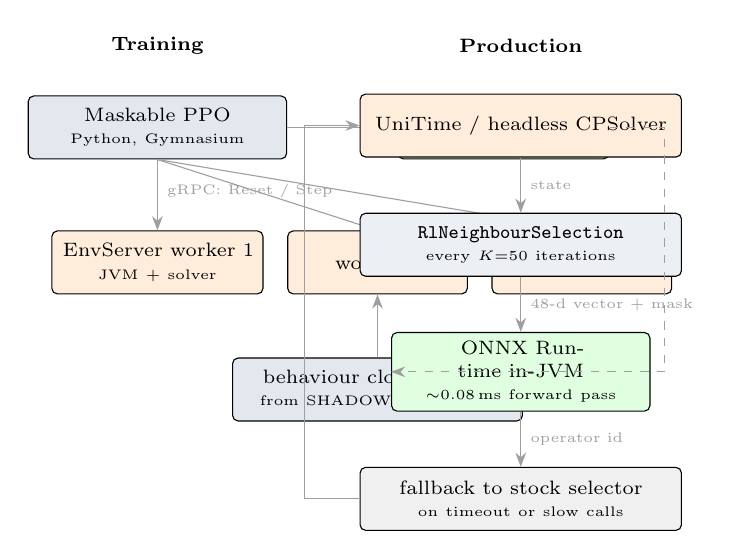
\begin{tikzpicture}[
  font=\small,
  blk/.style={draw,rounded corners=2pt,align=center,font=\scriptsize,minimum height=8mm,inner xsep=4pt},
  jvm/.style={blk,fill=orange!14},
  py/.style={blk,fill=coepblue!12},
  pol/.style={blk,fill=green!12},
  ar/.style={-{Stealth[length=1.8mm]},gray!75},
  lbl/.style={font=\scriptsize\bfseries}
]
% --- training
\node[lbl] (tl) {Training};
\node[py, below=4mm of tl, text width=30mm] (ppo) {Maskable PPO\\{\tiny Python, Gymnasium}};
\node[jvm, below=9mm of ppo, text width=24mm] (w1) {EnvServer worker 1\\{\tiny JVM + solver}};
\node[jvm, right=3mm of w1, text width=20mm] (w2) {worker 2};
\node[jvm, right=3mm of w2, text width=20mm] (w3) {worker 3};
\draw[ar] (ppo.south) -- node[right,font=\tiny,pos=0.45]{gRPC: Reset / Step} (w1.north);
\draw[ar] (ppo.south) -- (w2.north);
\draw[ar] (ppo.south) -- (w3.north);
\node[py, below=8mm of w2, text width=34mm] (bc) {behaviour cloning prior\\{\tiny from SHADOW trajectories}};
\draw[ar] (bc.north) -- (w2.south);
\node[pol, right=14mm of ppo, text width=24mm] (onnx) {export to ONNX\\{\tiny \texttt{policy.onnx}}};
\draw[ar] (ppo) -- (onnx);

% --- production
\node[lbl, right=30mm of tl] (pl) {Production};
\begin{scope}[xshift=84mm]
\node[jvm, below=4mm of pl, text width=38mm] (solver) {UniTime / headless CPSolver};
\node[blk, below=7mm of solver, text width=38mm, fill=coepblue!8] (rlns) {\texttt{RlNeighbourSelection}\\{\tiny every $K{=}50$ iterations}};
\node[pol, below=7mm of rlns, text width=30mm] (ort) {ONNX Runtime in-JVM\\{\tiny $\sim$0.08\,ms forward pass}};
\node[blk, below=7mm of ort, text width=38mm, fill=gray!12] (fb) {fallback to stock selector\\{\tiny on timeout or slow calls}};
\draw[ar] (solver) -- node[right,font=\tiny]{state} (rlns);
\draw[ar] (rlns) -- node[right,font=\tiny]{48-d vector + mask} (ort);
\draw[ar] (ort) -- node[right,font=\tiny]{operator id} (fb);
\draw[ar] (fb.west) -- ++(-7mm,0) |- (solver.west);
\end{scope}
\draw[ar,dashed] (onnx.east) -- ++(7mm,0) |- (ort.west);
\end{tikzpicture}
\caption{Training and production configurations of the learning layer. During training, Python
drives several resident JVM workers over gRPC; in production the frozen policy runs inside the
solver's own JVM with a fallback path.}
\label{fig:rl}
\end{figure}

\subsection{Evaluation design}

Five arms were defined so that any effect attributable to learning could be separated from effects
attributable to re-weighting or to a different search strategy.

\begin{table}[H]
\centering
\caption{Experimental arms.}
\label{tab:arms}
\footnotesize
\begin{tabular}{@{}clL{7.4cm}l@{}}
\toprule
\textbf{Arm} & \textbf{Role} & \textbf{Selector} & \textbf{Comparator} \\
\midrule
B0 & untuned baseline & \texttt{FixCompleteSolutionNeighbourSelection}, stock weights & native \\
B1 & tuned baseline   & as B0, with the student-conflict weight raised                & native \\
B2 & strategy control & \texttt{SimpleSearch} Great Deluge, student swap, suggestions  & native \\
L  & online learning  & the layer with LinUCB over the eight operators                & lexicographic \\
R  & frozen policy    & the layer with the exported ONNX policy                       & lexicographic \\
\bottomrule
\end{tabular}
\end{table}

Arm L uses LinUCB~\cite{li2010linucb}, a disjoint linear contextual bandit from the
upper-confidence-bound family~\cite{auer2002ucb}: it is an online, linear method, not a neural
network, and serves as a cheap learner that needs no pre-training. Arm R is the PPO-trained policy
frozen into ONNX. A sixth mode, SHADOW, executes the default selector while logging what the policy
\emph{would} have chosen, and supplies the trajectories for behaviour cloning.

\subsection{What was implemented, measured, and not established}

The layer is complete. Its central claim is not.

\paragraph{Implemented.} 25 Java classes and 11 Python modules: the neighbour-selection wrapper,
all eight operators, the incremental conflict oracle, the 48-feature encoder, four policy back-ends,
the headless runner, the gRPC environment and a synthetic instance generator. The oracle matches a
full recompute over 200 batches of random moves, and the exported ONNX graph matches the PyTorch
model.

\paragraph{Measured on synthetic data only.} On 120 classes, 600 students and 6 rooms, 30 seconds,
one seed, the pipeline runs end to end: about 100 macro-steps per second per worker, reset under a
second, an ONNX forward pass of about 0.08\,ms, and a PyTorch--ONNX deviation of $2\times10^{-6}$.
Every arm ties at $C = 0.133$ and the behaviour-cloned policy is worse, at $0.267$, having collapsed
onto one operator. The project's own notes call this a pipeline check, and so does this report.

\paragraph{Measured on real data.} Training ran for 100{,}000 timesteps on three workers over the
Spr6 instance and exported a policy. The only bake-off on a real instance covers B0, B1 and B2, and
that instance was already conflict-free when loaded, so it could not have separated the arms.

\paragraph{Not established.} No claim is made that the learned policy beats the baselines. Arms L
and R have never run on a COEP instance, and there is no held-out term.

\subsection{Outcome: the control answered the question}

Arm B1 exists to ask whether the objective was simply under-weighted, and
Section~\ref{sec:experiments} shows that it was. Raising the weight on a fixed instance took the
median violation rate from 0.0414 to 0.0030 or below, a reduction of over 90\,\%, well past the
25\,\% the learned policy had been set to beat. The sweep summary says so directly: the research
question is answered in the negative, and the learned run is optional.

That is a finding, not a failure. On this instance and this budget the residual conflicts came from
how the objective was priced, not from how the search explored, and a tuned stock solver is enough.
The oracle, the encoder and the headless runner stay useful: they are what made the controlled
comparison possible, and they are ready if a larger instance turns out not to yield to the weight.

\subsection{Risks}

Inference cost is limited by macro-stepping, the ONNX timeout and the fallback. A policy that
cheats by leaving classes unassigned is discouraged by the unassigned term in $\Phi$ and by a
callback that drops the gradient of any episode whose assigned ratio falls by more than five
points. Over-fitting to one term is not handled, which is why no generalisation claim is made.

\section{Implementation History and Codebase Overview}
\label{sec:history}

\subsection{Version history}

The repository contains 30 commits from 23 June 2026 to 8 October 2026, with two contributors. It
has no tags, and the version history was built from commit comments and dates rather than from
release markers. Table~\ref{tab:history} summarises the seven phases in the order they occurred,
with the labels used in the project's presentation material (the informal version).

\begin{table}[H]
\centering
\caption{Development phases reconstructed from the commit history.}
\label{tab:history}
\footnotesize
\begin{tabular}{@{}L{1.3cm}L{2.0cm}L{8.2cm}L{2.6cm}@{}}
\toprule
\textbf{Phase} & \textbf{Dates} & \textbf{Content} & \textbf{Deck label} \\
\midrule
1 & 23 Jun 2026 & Repository bootstrapped; first generators; first exported solutions. & v1 \\
2 & 29 Jul -- 22 Aug 2026 & Preference-based enrolment simulation; time-pattern update; elective
    lecture/lab pairing fix on the course offering import. & v2, v3, v5 \\
3 & 26--29 Aug 2026 & Constraint work: term advanced to Spr5, then to Spr6; minor-degree block
    scheduling; flexible time-preference rule engine; emission of matching slots, instead of
    blanket prohibitions; master pipeline \texttt{gen\_all.py}; lunch-break persistence repair;
    purge utility; renamed the first-year reserved course. & v4 \\
4 & 7--11 Sep 2026 & Full Taasika dump is added; snapshot 263 is integrated into the loader, with
    improvements to the KPI evaluation, and a room-preference toggle has been added. & --- \\
5 & 28 Sep 2026 & The reinforcement-learning module and the solution for Spring 2026 land directly
    in one commit, along with the setup guide via arm B1. & RL \\
6 & 29 Sep -- 1 Oct 2026 & Departmental and open-elective logic and curriculum correction; open
    elective that can only appear in second year; automatic archive generation; online rooms
    removed from generation; open-elective block enrolments added. & --- \\
7 & 8 Oct 2026 & Student group membership is based on enrolments. & --- \\
\bottomrule
\end{tabular}
\end{table}

The elective pairing fix is recorded in the handover notes as an offering reduction from 63 to 58:
five standalone laboratory offerings were absorbed into their lecture partners. An earlier note
said 63 reduced to 54. That 54 is not in the notes or in the files. The current dataset, after
the later curriculum edits, contains 56 offerings (Table~\ref{tab:dataset}). The phase structure
above is not necessarily in sync with the labels v1--v5, and is only loosely tied to the
individual commits.

\subsection{Repository layout}

\begin{table}[H]
\centering
\caption{Top-level repository structure.}
\label{tab:layout}
\footnotesize
\begin{tabular}{@{}L{3.0cm}L{11.9cm}@{}}
\toprule
\textbf{Path} & \textbf{Contents} \\
\midrule
\texttt{scripts/}     & 25 Python generators, validators and evaluators, and two Jython scripts in
                        \texttt{unitime\_scripts/} that execute inside UniTime \\
\texttt{unitime-out/} & Created XML for the generalised Data Exchange, the frozen dataset
                        \texttt{0gen\_all/} and the archive \\
\texttt{rl/}          & Maven module, Python training package, configuration, instance, models and
                        experiment runs for \texttt{unitime-rl} \\
\texttt{cpsolver/}    & Local copy of the CPSolver library, ready to be built and installed into
                        the module system \\
\texttt{solutions/}   & Exported timetables used on report sheets for the KPI reports to score \\
\texttt{taasika-db/}  & The institutional SQL dumps \\
\texttt{compare/}     & Snapshot summaries usable by humans to compare snapshots \\
\bottomrule
\end{tabular}
\end{table}

Figure~\ref{fig:arch} shows how these parts relate at run time.

\begin{figure}[H]
\centering
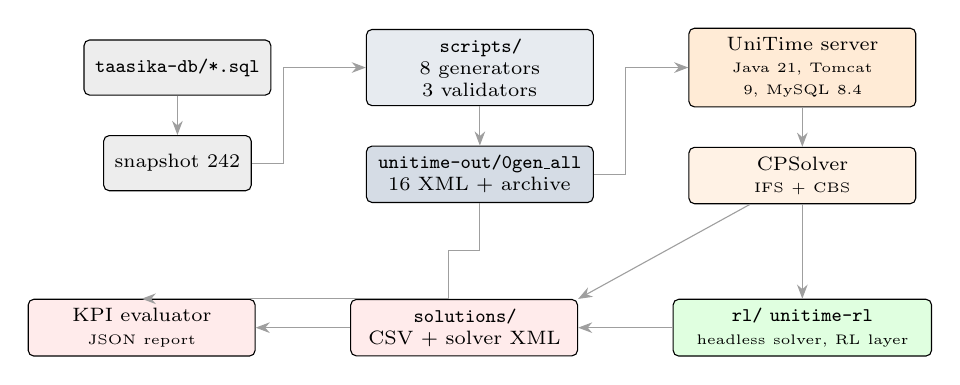
\begin{tikzpicture}[
  font=\scriptsize,
  grp/.style={draw,rounded corners=3pt,inner sep=5pt},
  blk/.style={draw,rounded corners=2pt,align=center,minimum height=7mm,inner xsep=4pt},
  ar/.style={-{Stealth[length=1.8mm]},gray!75}
]
% data layer
\node[blk,fill=gray!14] (sql) {\texttt{taasika-db/*.sql}};
\node[blk,fill=gray!14,below=5mm of sql] (snap) {snapshot 242};

% generation layer
\node[blk,fill=coepblue!10,right=12mm of sql,text width=26mm] (scripts) {\texttt{scripts/}\\8 generators\\3 validators};
\node[blk,fill=coepblue!18,below=5mm of scripts,text width=26mm] (xml) {\texttt{unitime-out/0gen\_all}\\16 XML + archive};

% unitime
\node[blk,fill=orange!16,right=12mm of scripts,text width=26mm] (ut) {UniTime server\\{\tiny Java 21, Tomcat 9, MySQL 8.4}};
\node[blk,fill=orange!10,below=5mm of ut,text width=26mm] (cps) {CPSolver\\{\tiny IFS + CBS}};

% rl
\node[blk,fill=green!12,below=12mm of cps,text width=30mm] (rl) {\texttt{rl/} \texttt{unitime-rl}\\{\tiny headless solver, RL layer}};

% outputs
\node[blk,fill=red!8,left=12mm of rl,text width=26mm] (sol) {\texttt{solutions/}\\CSV + solver XML};
\node[blk,fill=red!8,left=12mm of sol,text width=26mm] (kpi) {KPI evaluator\\{\tiny JSON report}};

\draw[ar] (sql) -- (snap);
\draw[ar] (snap.east) -- ++(4mm,0) |- (scripts.west);
\draw[ar] (scripts) -- (xml);
\draw[ar] (xml.east) -- ++(4mm,0) |- (ut.west);
\draw[ar] (ut) -- (cps);
\draw[ar] (cps) -- (sol.north east);
\draw[ar] (cps) -- (rl);
\draw[ar] (rl) -- (sol);
\draw[ar] (sol) -- (kpi);
\draw[ar] (xml.south) |- ++(-4mm,-6mm) |- (kpi.north);
\end{tikzpicture}
\caption{The \texttt{scripts/} generators and validators read the Taasika SQL dump (snapshot 242)
and create the 16 XML files and archive in \texttt{unitime-out/0gen\_all}. That output goes to the
UniTime server (Java 21, Tomcat 9, MySQL 8.4) using CPSolver (IFS + CBS), and also to the headless
\texttt{unitime-rl} module with the RL layer. Both solve one XML and write CSV and solver XML to
\texttt{solutions/}. The KPI evaluator scores those solutions against the same XML and returns a
JSON report.}
\label{fig:arch}
\end{figure}

\subsection{The generation and solving procedure}

The procedure actually followed is the one below, in the style of the corresponding section of the
Semester~VI report but updated for the current tooling.

\begin{enumerate}
  \item \textbf{Generate.} \texttt{python scripts/gen\_all.py --term Spr12 --sql
    taasika-db/taasika3.sql --snapshot 242}, the same command as
    Listing~\ref{lst:genall}. The eight generators are dependent on one another.
  \item \textbf{Validate and archive.} The same command runs the three validators and writes
    \texttt{0gen\_all.zip} if all three pass.
  \item \textbf{Import.} Upload the archive through Data Exchange; it uploads files 1--16 one by
    one.
  \item \textbf{Attach buildings and teachers.} Run \textbf{Buildings\,$\rightarrow$\,Update
    Data}. There is no need to send any data at this point merely because a building has no room,
    or each building reports that it does not have room. Add staff through \textbf{Manage
    Instructor List}.
  \item \textbf{Lunch breaks.} Run \texttt{setup\_lunch\_breaks.py} under
    \textbf{Utilities\,$\rightarrow$\,Scripts}.
  \item \textbf{Pin enrolments.} Set up the three functions of Section~\ref{sec:setup}.
  \item \textbf{Check, solve, export.} Run with the \texttt{Check} configuration. It cycles through
    all classes and prints the loaded classes and the number of students loaded (there must be at
    least one). Load in \texttt{Initial} mode, then solve and export CSV until the timeout occurs.
    If the solver XML is to be exported, set \texttt{unitime.solution.export.names=true}
    beforehand.
  \item \textbf{Evaluate and refine.} Repeat the steps above for the same dataset, and score with
    \texttt{eval\_timetable\_kpis.py} using the check to be fixed.
\end{enumerate}

\subsection{The most recent change: enrolment-derived group membership}

In the last commit of the phase, the way student groups are populated was changed. In the past the
data had been reported as 242 groups, back-filled as empty groups, since bulk updates of the
groups caused a Hibernate failure while importing the data. The generator now operates on
enrolments: membership of a class is determined by the schedule note for that class, and this is
emitted as a group reference for that class within the student's record in file 14. If a note is
not recognised it is dropped and not imported. The codes are checked against the codes declared in
file 6.

The result is 5{,}767 group references from 1{,}130 students, verified exhaustively: each student
enrolled in a class is part of the group of that class, for all classes, with no unrecognised code
and well-formed output. As Section~\ref{sec:constraints} explains, this is possible without
altering the timetable, so the cohort structure is visible. With the pinning flags applied, 40
conflicts were present after the change.

\section{Limitations}
\label{sec:limitations}

Conditions for the results of Section~\ref{sec:experiments} should be clearly stated.

\paragraph{Student population is emulated.} There was no MIS data available, so all 1{,}130 students
are based on confirmed headcounts and deterministic rules for enrolment. The number of cohorts,
their divisions and the size of the batches is reasonable, but the selection of courses is not a
genuine choice. In fact, elective demand is assumed to be even but real elective demand is skewed,
and if it is, then more students would belong to the larger sections and its overlaps would become
more significant.

\paragraph{Defects in the data that is created.} Since the declared sections do not include two
hundred first year students, two hundred of them could not be accommodated in
\texttt{CS PPS-FY Lec}. The \texttt{PSEC2-EAI} laboratory is a crowded place with tech students.
After all the sections are filled due to the order of filling the sections, three final year
laboratory batches are made up of two different lecture divisions inadvertently, which are not the
institution's intention. There are no members in the groups \texttt{BT-Div1}, \texttt{BT-Div2} and
\texttt{FY-PP1-A\_}. The first-year programming lab sections (16--41) are still present in the
offering file and will be deleted again in an incremental import, even if they are not desired,
thus it is necessary to re-import the file after an unmatching of any saved solution, so that the
classes in these sections are not deleted.

\paragraph{Scope is a department and a term.} All information stated here applies to the Spring
2026 class for the Department of Computer Engineering. The size of a university-wide instance
would be several times bigger and would add inter-departmental room contention which this dataset
does not cover.

\paragraph{The war is still alive and kicking.} The first 40 conflicts were diagnosed and
localised in four laboratory placements to the reserved lecture block, but were never corrected.
Two remedies were noted, one being to re-time those laboratories, or to add explicit different-time
distribution constraints between those laboratories and those reserved block, but have not yet been
implemented or measured.

\paragraph{The quality of the soft constraints is low.} The room preference hit rate is
12.59\,\%, and 17 of 291 assignments end up in the pool of unavailable laboratory. The solver is
using the hard constraints and using up their soft budget. No effort was made to tune the
room-preference weight.

\paragraph{The evaluator presents the evaluator's broken check.} The instructor identity check
scores are all 0\,\% because they do not match a name that is formatted differently; that column
of the preference score has no information and brings down the average. There should therefore not
be a single interpretation of the overall preference score of 6.29.

\paragraph{The learning layer has never been implemented with real data.} The only bake-off that
ran on real data covered the three baselines and was run on an instance that was already
conflict-free, and Arms L and R have never been run on a COEP instance. No statement on
generalisation is possible since there is no held-out term, and training was performed using just
one instance. The performance numbers provided in the layer are for a synthetic instance of 120
classes.

\paragraph{There is one experimental artefact that is not consistent.} There is a discrepancy
between the recorded summary and the per-seed metric files for weight 5. The sweep stores 21
files, three seeds at each of seven configurations, and weight 5 has three of them, not fifteen.
One of those three appears to have been repeated after the summary was written. Both
readings appear in Section~\ref{sec:experiments} and neither alters the conclusion, but the run
was not repeated to make a decision.

\paragraph{Provenance records in the dataset are incorrect in the files.} Four of the documents
generated have hard-coded attributes that refer to snapshot 240, and the dataset generated refers
to snapshot 242. The entities had to be counted to reconstruct the provenance. The generators
should record the snapshot that they were handed.

\paragraph{There is no teacher version interface.} The Taasika snapshot is read to get information
about the availability and preferences of the instructor. The interface which was proposed in
Semester~VI that would allow the staff to enter their own constraints has not been developed and
hence the preference data is only as up to date as the snapshot.

\section{Future Scope}
\label{sec:future}

\subsection{Status of the items carried over from Semester VI}

Table~\ref{tab:carryover} revisits every direction proposed in the previous report and records what
the present phase did with it.

\begin{table}[H]
\centering
\caption{Semester VI proposals and their current status.}
\label{tab:carryover}
\footnotesize
\begin{tabular}{@{}L{4.4cm}L{2.2cm}L{8.3cm}@{}}
\toprule
\textbf{Proposal} & \textbf{Status} & \textbf{Position at the end of Semester VII} \\
\midrule
Examination scheduling & still open &
  Examination periods are declared in \texttt{1sessionSetup.xml}, but no per-course examination
  elements are emitted and the examination module has not been exercised. Taasika does not model
  examinations, so the data would have to come from elsewhere. \\
Calendar (\texttt{.ics}) integration & still open &
  Not started. The exported CSV contains everything a calendar export needs, so this is now a
  self-contained task rather than one blocked on the timetable. \\
University-wide deployment & still open &
  The pipeline is parameterised by snapshot and term and is not specific to one department, but
  only Computer Engineering data has been loaded and solved. \\
Automated change notification & still open & Not started. \\
WhatsApp group automation & still open & Not started. \\
Student data pipeline from the MIS portal & partly done &
  The transformation and import path is built, validated and exercised end to end, producing
  1{,}130 student records with 9{,}148 enrolments. Only the data source is missing: the generator
  simulates students because MIS extracts were not available. Substituting the real source is a
  change to one generator. \\
Course definition interface for instructors & partly done &
  Course, section and preference generation is fully automated from the Taasika snapshot, so no
  manual data entry is required. The instructor-facing interface for submitting availability has
  not been built. \\
Constraint mapping onto UniTime & done &
  Established in Semester VI and now implemented as generated data rather than as a mapping on
  paper (Section~\ref{sec:constraints}). \\
Handling of shared multi-instructor laboratories & partly done &
  Multiple lead instructors on one class is supported by UniTime and used, but the stronger
  requirement---two instructors blocked simultaneously for the same student set in the same
  room---has no distribution constraints generated for it. \\
\bottomrule
\end{tabular}
\end{table}

\subsection{New directions arising from this phase}

\begin{enumerate}
  \item \textbf{Resolve the residual first-year conflicts.} The 40 remaining conflicts are
    concentrated in four laboratory placements against the reserved first-year lecture block.
    Adding generated different-time distribution constraints between the programming laboratory
    subpart and the reserved block would make the requirement explicit to the solver rather than
    leaving it to the student-conflict weight. This is the smallest remaining step with a direct
    effect on the headline metric.

  \item \textbf{Student sectioning with pre-defined batches.} The institution assigns batches
    administratively, which is why student switching had to be disabled. The principled alternative
    is to express the batches as group reservations, so that UniTime may section students but only
    within the batch they belong to. This would recover the solver's freedom to resolve conflicts
    by sectioning without discarding the cohort structure.

  \item \textbf{Soft-constraint optimisation.} The room preference hit rate of 12.59\,\% is the
    weakest measured quantity. Work is needed on both sides: tightening the generated preferences,
    which are currently permissive, and tuning the room-preference weight against the
    student-conflict weight in the manner of the sweep in Section~\ref{sec:experiments}.

  \item \textbf{Fix and extend the evaluator.} Normalising instructor names would repair the
    identity check and make the preference score meaningful. Replacing the exact-slot matching in
    \texttt{sectioning\_slot\_conflicts.py} with the interval test used elsewhere would remove a
    tool that currently reports false negatives.

  \item \textbf{One-command snapshot to solution.} Generating, importing, solving and evaluating
    currently requires three scripts and several manual steps in the UniTime interface. Since the
    headless solver can already load a solver XML and solve it outside the server, an end-to-end
    command from a Taasika snapshot to a scored solution is achievable and would make the
    refinement loop of Section~\ref{sec:evaluation} substantially faster.

  \item \textbf{Write the solution back to Taasika.} The timetable is currently a dead end: it is
    exported as CSV and XML but never returned to the system the institution actually uses. A
    converter from a solved timetable into the Taasika snapshot format would close the loop and is
    a precondition for the system being adopted operationally.

  \item \textbf{Complete the learning-layer evaluation, or retire it.} Arms L and R should be run
    against arm B1 on a held-out term, at equal wall-clock budget, on an instance that is not
    already conflict-free. If a harder instance---a university-wide one, for example---proves
    resistant to weight tuning, the layer is ready to be evaluated on it. If no such instance
    appears, the honest conclusion of Section~\ref{sec:rl} stands and the layer should be kept as
    instrumentation rather than as a solver component.

  \item \textbf{Correct the dataset defects.} The unplaced first-year cohort, the over-subscribed
    M.Tech laboratory, the cross-division batches, the empty groups and the obsolete laboratory
    sections 16--41 are all input-data problems with known fixes, and each removes a source of
    spurious conflicts.
\end{enumerate}

\section{Conclusion}
\label{sec:conclusion}

In the Semester~VI part of this project, it was concluded that it is possible to represent any
scheduling rule used at COEP Technological University within UniTime's constraint model. This is a
statement concerning the platform. The current phase (in the name of the project
\emph{taasika-v3}) made it a functional system and in the process created a quantified time plan
rather than a feasibility case.

Three objects were constructed. Behind three validators, and a single command, a reproducible
pipeline reads a snapshot of the institution's existing Taasika database and generates the sixteen
ordered documents that UniTime requires: the session, the curriculum, 42 rooms (across 6
buildings), 115 instructors, 56 offerings (291 classes), and a simulated body of 1{,}130 students
(9{,}148 section enrolments). The minor-degree and open-elective block times are also produced as
data and the dynamic lunch window for students and teachers is also generated as data---the
institution's own rules are generated as data not re-entered after every import. Any exported
timetable is independently scored by an evaluator working with the same input files against a
definition of a conflict which was cross-validated with another implementation to obtain exact
agreement.

The substantive outcome of the phase is more about measurement than optimisation. A number of
configurations reported no conflicts among students, and each of these was traced to either a
``no student'' situation, meaning that the solver loaded no students, or a ``no student'' being
re-sectioned between student batches, which is already ``no conflict''. They found that when they
pin the enrolments (\emph{Enrolled Student Course Demands}, disable student switching, and load
enrolments from the stored solution), the solver can no longer improve the number and the number
reported actually increased from what they thought was zero to 40. That was the goal they set for
themselves. The final solution has 290 of 291 classes with no instructor, no room double booking,
which is a hard feasibility score of 98.85 out of 100 and 40 of 1{,}130 students conflicted, all
of which were first year students in four laboratory placements with one reserved lecture block.
The residue is not diffuse, it is concentrated and thus a scheduling problem rather than a ceiling
on quality.

The reinforcement-learning layer is not entirely inside the solver JVM. Training is the 11 Python
modules and the gRPC environment. Production inference is the 25 Java classes and the ONNX path
inside the JVM. The layer never returns an illegal timetable, because the stock CPSolver generates
and accepts every move. The weight sweep lowered the median violation rate on a fixed instance
from 0.0414 to 0.0030 at weight 2, the best weight on disk. That is not the pre-registered
comparison: the 25\,\% bar was a learned policy against a tuned baseline on a held-out instance,
and that comparison was not run. It is not claimed that the learned policy performs better than
the baselines, as arms L and R were not run on institutional data, and there is no held-out term. The helpful ending is much more restrictive: in this case, the
leftover student conflicts were the result of the pricing of the objective rather than of the
search's exploration, and a properly configured stock solver will do the job. The layer's conflict
oracle, state encoder and headless runner remain useful as instrumentation for that comparison,
which has not been run.

So the institution now has a way to get from their live scheduling database to a scored timetable
that can be re-run whenever they want, and their scored number is honest. It doesn't yet have a
return route: the solution is exported but not written back to Taasika, the student data is
simulated and not pulled from the MIS portal, the scope is one department for one term. Those are
the three steps between the present system and its use as an operating system, and they are now
statements of fact and not questions.


% ============================================================ APPENDICES
\appendix
\renewcommand{\thesection}{\Alph{section}}
\section{The Sixteen XML Imports}
\label{app:imports}

Each document references entities created by an earlier one, so the numbering is the import order.
The archive must hold the files at its root, and the Data Exchange term is the academic term
followed by the year (\texttt{Spr122026}).

\begin{longtable}{@{}rL{4.7cm}L{10.0cm}@{}}
\caption{The sixteen Data Exchange documents and their dependencies.}
\label{tab:imports}\\
\toprule
\textbf{\#} & \textbf{File} & \textbf{Creates, and what it requires} \\
\midrule
\endfirsthead
\multicolumn{3}{@{}l}{\small\itshape Table~\thetable\ continued.}\\
\toprule
\textbf{\#} & \textbf{File} & \textbf{Creates, and what it requires} \\
\midrule
\endhead
\bottomrule
\endfoot
1  & \texttt{1sessionSetup.xml}           & Session, departments, subject areas, date and time patterns. Nothing can precede it. \\
2  & \texttt{2academicArea.xml}           & Two areas, B.Tech and M.Tech. Requires the session. \\
3  & \texttt{3academicClassification.xml} & Five year codes: FY, SY, TY, BT, MT. \\
4  & \texttt{4Major.xml}                  & Fifteen majors. Requires file 2. \\
5  & \texttt{5Minor.xml}                  & Empty: Taasika models minors as majors. Requires file 2. \\
6  & \texttt{6studentGroup.xml}           & 242 groups, one per class and per batch. Must precede file 14. \\
7  & \texttt{7buildingRoomImport.xml}     & Six buildings, 42 rooms. Buildings are global and must then be attached with \textbf{Buildings\,$\rightarrow$\,Update Data}. \\
8  & \texttt{8roomSharing.xml}            & Department assignment; weekends unavailable. Requires file 7. \\
9  & \texttt{9travelTimes.xml}            & Five minutes between buildings, three between the two CSE buildings. \\
10 & \texttt{10staff.xml}                 & 115 instructors. Also needs \textbf{Manage Instructor List} before they attach to classes. \\
11 & \texttt{11courseCatalog.xml}         & 158 courses; paired laboratories merged into their lecture. Requires file 1. \\
12 & \texttt{12courseOffering.xml}        & 56 offerings, 84 subparts, 291 classes, times left blank. Requires files 10 and 11. \\
13 & \texttt{13preferences.xml}           & Time pattern, date pattern and room preferences on every subpart. Without it classes do not load. Re-import whenever file 12 changes. \\
14 & \texttt{14studentInfo.xml}           & 1{,}130 students and 5{,}767 group references. Requires files 2--4 and 6. \\
15 & \texttt{15studentRequest.xml}        & Course requests for all 1{,}130 students. Requires files 11 and 14. \\
16 & \texttt{16studentenrollments.xml}    & 9{,}148 section enrolments, the rows read under \emph{Enrolled Student Course Demands}. Requires files 12 and 14. \\
\end{longtable}

\noindent The Jython utility \texttt{purge\_uploaded\_data.py} deletes a chosen subset of these
steps (\texttt{"16"}, \texttt{"12, 13"}, \texttt{"14-16"}) in reverse dependency order.

\section{Spr6 Instance Inventory}
\label{app:spr6}

The Spr6 session is the instance behind every headless experiment in Section~\ref{sec:experiments}
and Section~\ref{sec:rl}. It is recorded separately from the current dataset because its counts
differ, and because quoting a conflict rate without the instance it came from was the single
largest source of confusion during the phase.

\subsection{The solver instance}

\begin{table}[H]
\centering
\caption{Properties of \texttt{rl/instances/spr2026.xml}.}
\label{tab:spr6inst}
\footnotesize
\begin{tabular}{@{}L{5.6cm}L{8.6cm}@{}}
\toprule
\textbf{Property} & \textbf{Value} \\
\midrule
Format            & CPSolver solver-model XML, \texttt{<timetable version="2.5">} \\
Origin            & \emph{Export XML} on the UniTime course timetabling solver screen \\
Session           & Spr6, 2026 \\
Classes (variables) & 262 \\
Students          & 990, carrying 7{,}748 enrolments \\
Rooms indexed     & 44 \\
Initial conflict rate & $C = 0.5313$ (526 of 990 students) \\
Self-contained    & Yes: rooms, instructors, time and room domains, distribution constraints,
                    students and the current assignment are all inside the file \\
\bottomrule
\end{tabular}
\end{table}

This format is \emph{not} produced by Data Exchange, whose timetable export is the class-assignment
interchange format and cannot be loaded by the solver. Two settings matter when producing it:
\emph{Student Course Demands} must be \emph{Enrolled Student Course Demands}, or the student block
is empty, and \texttt{unitime.solution.export.names} must be \texttt{true}, or class and room names
are stripped.

\subsection{Derived artefacts}

\begin{table}[H]
\centering
\caption{Artefacts derived from the Spr6 session.}
\label{tab:spr6art}
\footnotesize
\begin{tabular}{@{}L{5.4cm}L{2.0cm}L{7.0cm}@{}}
\toprule
\textbf{Artefact} & \textbf{Type} & \textbf{Role} \\
\midrule
\texttt{rl/instances/spr2026.xml}            & solver XML & the instance above; input to every sweep run \\
\texttt{rl/instances/spr2026-nostudents.xml} & solver XML & the same export before student injection \\
\texttt{rl/instances/spr2026v6\_mihir.xml},
  \texttt{spr2026v8\_mihir.xml}              & solver XML & later exports of the same session \\
\texttt{solutions/spr2026.kpi.json}          & KPI report & scores the instance: 526/990, hard feasibility 92.15 \\
\texttt{solutions/COEPSpr62026\_v2.csv}      & CSV        & exported timetable, scored in \texttt{kpi\_report.json} \\
\texttt{solutions/course-solution\_weight5.csv},
  \texttt{\_weight20.csv}                    & CSV        & the UniTime weight experiments of Section~\ref{sec:experiments} \\
\texttt{solutions/spr2026\_10m\_w5.csv}      & CSV        & ten-minute run at weight 5 \\
\texttt{rl/runs/sweep/}                      & run tree   & the controlled weight sweep: 7 configurations $\times$ 3 seeds \\
\texttt{rl/runs/bakeoff-spr2026\_10m\_w5/}   & run tree   & arms B0, B1, B2 $\times$ 10 seeds on an already-solved instance \\
\texttt{rl/runs/sweep/w5/.../solution.xml}   & solver XML & scored independently in \texttt{solutions/solution.kpi.json} \\
\bottomrule
\end{tabular}
\end{table}

\subsection{Why 990 and not 1{,}290}

The dataset of this period declared 1{,}290 simulated students. The solver export carries 990. The
difference is not attrition: 990 is the number of students for whom the solver had loaded
enrolments at the moment of export. A conflict rate computed over 990 and one computed over
1{,}290 are therefore measurements of different populations, which is why
Table~\ref{tab:crossrun} records the denominator for every run.

\section{KPI Definitions}
\label{app:kpis}

All definitions below are as implemented in \texttt{scripts/eval\_timetable\_kpis.py}. Let $A$ be
the set of assigned classes in the solution, $S$ the set of students in the enrolment data, and
for a student $s$ let $E(s)$ be the set of assigned classes $s$ is enrolled in.

\subsection{The overlap predicate}

Two classes $c_1, c_2$ overlap, written $\mathrm{ov}(c_1,c_2)$, if and only if all three hold:

\begin{enumerate}
  \item they share at least one day: $\mathrm{days}(c_1) \land \mathrm{days}(c_2) \neq 0$, where
    days are a seven-bit mask with index 0 = Monday;
  \item their slot intervals intersect:
    $\mathrm{start}(c_1) < \mathrm{end}(c_2) \;\wedge\; \mathrm{start}(c_2) < \mathrm{end}(c_1)$,
    so intervals that merely touch at an endpoint do \emph{not} overlap;
  \item if both carry date patterns, the patterns share at least one active week.
\end{enumerate}

Room and instructor play no part in the test. Slots are five minutes when the session declares 288
slots per day.

\subsection{Hard checks}

Each check reports \emph{checked}, \emph{passed}, \emph{failed} and a pass rate, together with up
to eight example failures.

\begin{table}[H]
\centering
\caption{The ten hard checks.}
\label{tab:hardkpi}
\footnotesize
\begin{tabular}{@{}L{3.5cm}L{11.4cm}@{}}
\toprule
\textbf{Check} & \textbf{Definition} \\
\midrule
\texttt{coverage} &
  Fraction of classes declared in the offering file that carry an assignment in the solution. \\
\texttt{time\_pattern\_fidelity} &
  Fraction of assigned classes whose number of meetings and minutes per meeting match the time
  pattern declared for their subpart. \\
\texttt{date\_pattern} &
  Fraction of assigned classes whose date pattern matches the one declared in the preference file. \\
\texttt{room\_capacity} &
  Fraction of assigned classes whose enrolment limit does not exceed the capacity of the assigned
  room. \\
\texttt{lunch\_weekend} &
  Fraction of assigned classes that do not fall on a weekend or inside a blocked slot. \\
\texttt{room\_unavailable} &
  Fraction of assigned classes placed in a room that is available at that time (XML mode). \\
\texttt{instructor\_lunch\_breaks} &
  Fraction of instructors who retain at least one free 60-minute window within 11:30--15:30 on
  every teaching day. \\
\texttt{student\_lunch\_breaks} &
  The same test applied to each student's combined timetable. \\
\texttt{instructor\_double\_booking} &
  Fraction of classes not overlapping another class with the same instructor. \\
\texttt{room\_double\_booking} &
  Fraction of classes not overlapping another class in the same room. \\
\texttt{student\_conflicts} &
  Fraction of students $s \in S$ for which no pair $c_1,c_2 \in E(s)$ satisfies
  $\mathrm{ov}(c_1,c_2)$. \\
\bottomrule
\end{tabular}
\end{table}

\subsection{Student conflict quantities}

Four related quantities are reported and must not be interchanged:

\begin{align*}
  \text{students\_with\_conflict} &= \bigl|\{\, s \in S \;:\; \exists\, c_1,c_2 \in E(s),\;
      \mathrm{ov}(c_1,c_2) \,\}\bigr| \\[2pt]
  \text{student\_conflict\_pairs} &= \bigl|\{\, (s,c_1,c_2) \;:\; c_1,c_2 \in E(s),\;
      \mathrm{ov}(c_1,c_2) \,\}\bigr| \\[2pt]
  C &= \frac{\text{students\_with\_conflict}}{\bigl|\{\, s : |E(s)| \ge 2 \,\}\bigr|}
      \qquad\text{(violation rate, students at risk)} \\[2pt]
  C_{\mathrm{checker}} &= \frac{\text{students\_with\_conflict}}{|S|}
      \qquad\text{(violation rate over all students)}
\end{align*}

$C$ and $C_{\mathrm{checker}}$ coincide whenever every student is enrolled in at least two classes,
which is true of the current dataset. Section~\ref{sec:experiments} reports $C$.

\subsection{Preference checks}

\begin{itemize}
  \item \texttt{room\_preference}: fraction of assigned classes placed in a room that appears in
    the class's preferred-room list.
  \item \texttt{instructor\_identity}: fraction of assigned classes whose instructor matches the
    one expected from the source data. \emph{This check is currently unreliable} because the two
    sides use different name formats (Section~\ref{sec:evaluation}).
  \item \texttt{unav\_onl}: count and percentage of assignments landing in the unavailable or
    online room pools.
\end{itemize}

\subsection{Aggregate scores}

Both aggregates are equal-weight means of the component pass rates, on a 0--100 scale:
\[
  \text{hard feasibility} = \frac{100}{|H|}\sum_{h \in H} r_h ,
  \qquad
  \text{preference score} = \frac{100}{|P|}\sum_{p \in P} r_p ,
\]
where $H$ is the set of hard checks and $P$ the set of preference checks, and $r$ is a pass rate in
$[0,1]$. Because the weights are equal, a single broken check moves the aggregate substantially;
the component rates should always be read alongside it.

\subsection{Efficiency metrics}

These are descriptive and carry no pass/fail threshold:

\begin{itemize}
  \item \textbf{Instructor weekly load}: mean, standard deviation, minimum and maximum of assigned
    minutes per week per instructor.
  \item \textbf{Travel violations}: consecutive classes for one student or instructor in buildings
    further apart than the gap between them permits.
  \item \textbf{Slot spread}: proportion of assignments in the early, middle and late thirds of the
    teaching day.
  \item \textbf{Back-to-back density}: proportion of assignments immediately adjacent to another
    class for the same instructor or cohort.
  \item \textbf{Unavailable/online usage}: share of assignments in those room pools.
\end{itemize}

\section{Evidence Table}
\label{app:evidence}

Every numeric claim in this report is traceable to a file in the repository. ``Verified'' means the
quantity was recomputed from the named file while preparing this report; ``file'' means it is
quoted from a committed artefact without re-running the command that produced it.

{\footnotesize
\begin{longtable}{@{}L{6.2cm}L{6.4cm}L{2.2cm}@{}}
\caption{Source for each claim made in this report.}
\label{tab:evidence}\\
\toprule
\textbf{Claim} & \textbf{Source} & \textbf{Status} \\
\midrule
\endfirsthead
\multicolumn{3}{@{}l}{\small\itshape Table~\thetable\ continued from the previous page.}\\
\toprule
\textbf{Claim} & \textbf{Source} & \textbf{Status} \\
\midrule
\endhead
\bottomrule
\endfoot

\multicolumn{3}{@{}l}{\textbf{Dataset (Section~\ref{sec:datasets})}}\\
56 offerings, 84 subparts, 291 classes & \texttt{0gen\_all/12courseOffering.xml} & verified \\
158 courses & \texttt{0gen\_all/11courseCatalog.xml} & verified \\
242 student groups & \texttt{0gen\_all/6studentGroup.xml} & verified \\
6 buildings, 42 rooms & \texttt{0gen\_all/7buildingRoomImport.xml} & verified \\
115 instructors & \texttt{0gen\_all/10staff.xml} & verified \\
1{,}130 students, 5{,}767 group references & \texttt{0gen\_all/14studentInfo.xml} & verified \\
9{,}148 section enrolments & \texttt{0gen\_all/16studentenrollments.xml} & verified \\
Term \texttt{Spr122026} & \texttt{term}/\texttt{year} attributes of all 16 files & verified \\
FY 400, SY/TY/BT 200, MT 130 & \texttt{solutions/enrollment\_sim\_summary.json} & file \\
200 unplaced in \texttt{PPS-FY Lec}; 2 in \texttt{PSEC2-EAI Lab} & same & file \\
Source snapshot 242 (\texttt{published-v4-26jan26}) & \texttt{compare/242.txt} vs.\ group and staff counts & verified \\
Session 19 Jan--22 May 2026; classes end 30 Apr; exams 4 May & \texttt{0gen\_all/1sessionSetup.xml} & verified \\

\multicolumn{3}{@{}l}{\textbf{Constraints (Section~\ref{sec:constraints})}}\\
Four fixed time-block rules & \texttt{scripts/gen\_preferences.py}, \texttt{FIXED\_ENTRIES\_MAP} & verified \\
Time-pattern mapping & \texttt{gen\_preferences.py}, \texttt{\_time\_pattern()} & verified \\
Ten declared time patterns & \texttt{0gen\_all/1sessionSetup.xml} & verified \\
Lunch break 11:30--15:30, dynamic & \texttt{unitime\_scripts/setup\_lunch\_breaks.py} & file \\
Group code = class schedule note; 289 notes & \texttt{scripts/offering\_index.json} & verified \\
Intake headcounts & \texttt{scripts/intake.py} & verified \\

\multicolumn{3}{@{}l}{\textbf{Final solution (Section~\ref{sec:experiments})}}\\
291 classes, 290 assigned, coverage 99.66\,\% & \texttt{eval\_timetable\_kpis.py} on \texttt{spr2026\_11\_all\_flags.csv} & verified \\
Hard feasibility 98.85; 4{,}341 checks, 105 failures & same & verified \\
0 instructor and 0 room double-bookings & same & verified \\
\textbf{40 of 1{,}130 students, 40 pairs} & same & verified \\
63 student and 1 instructor lunch violations & same & verified \\
Room preference 12.59\,\%; 17 of 291 unavailable/online & same & verified \\
Instructor identity 0\,\% is a name-format artefact & example rows in the same report & verified \\
All 40 conflicts are \texttt{PPS-FY Lab} $\times$ \texttt{FY-Reserve Lec} & failure examples in the same report & verified \\

\multicolumn{3}{@{}l}{\textbf{Weight experiments (Section~\ref{sec:experiments})}}\\
Weight 5: 676 of 1{,}290; 1{,}076 pairs & \texttt{solutions/kpi\_weight5\_report.json} & file \\
Weight 20: 894 of 1{,}290; 2{,}126 pairs & \texttt{solutions/kpi\_weight20\_report.json} & file \\
Sweep medians (Table~\ref{tab:sweep}) & \texttt{rl/runs/sweep/summary.md}, \texttt{sweep\_results.csv} & file \\
B0 median $C=0.0414$ (seeds 0.0414, 0.0263, 0.0515) & \texttt{rl/runs/sweep/B0/.../metrics.json} & verified \\
Initial $C = 0.5313$ (526 of 990) & \texttt{initial.student\_violation\_rate} in all sweep runs & verified \\
Weight-5 row inconsistency & \texttt{w5/.../seed1/metrics.json} vs.\ \texttt{sweep\_results.csv} & verified \\
900\,s budget, 3 seeds, 262 variables assigned & \texttt{metrics.json} of each run & verified \\

\multicolumn{3}{@{}l}{\textbf{Measurement reconciliation (Sections~\ref{sec:evaluation},~\ref{sec:experiments})}}\\
Solver checker 526/990 = 53.1\,\% & \texttt{solutions/spr2026.kpi.json} & file \\
KPI evaluator 587/1{,}290 = 45.5\,\% & \texttt{solutions/kpi\_report.json} & file \\
Java oracle 0.026262626 vs.\ Python 0.026263 & \texttt{w5/.../seed1/metrics.json}, \texttt{solutions/solution.kpi.json} & verified \\
Bake-off instance already at $C=0$ on load & \texttt{bakeoff-spr2026\_10m\_w5/.../metrics.json} & verified \\
\texttt{spr2026\_10\_LE\_90m\_w5} loaded 0 students & \texttt{meta.enrolled\_students = 0} in its KPI report & verified \\
Pinned Spr10 run: 32 of 1{,}130 & \texttt{solutions/spr2026\_10\_LE\_SS\_Enrolled.kpi.json} & file \\

\multicolumn{3}{@{}l}{\textbf{Learning layer (Section~\ref{sec:rl})}}\\
25 Java classes & \texttt{rl/src/main/java/.../rl/} & verified \\
11 Python modules & \texttt{rl/python/unitime\_rl/} & verified \\
48-dimensional state; feature names & \texttt{StateEncoder.java}, \texttt{DIM}, \texttt{NAMES} & verified \\
Eight operators and their ids & \texttt{Operators.java} & verified \\
$K = 50$; reward $\Phi$; masking rules & \texttt{rl/README.md}, \texttt{RlConfig.java} & file \\
PPO: 100{,}000 timesteps, 3 workers, BC init & \texttt{rl/models/ppo/train\_args.json} & verified \\
Synthetic smoke-test figures & \texttt{rl/README.md}, ``Smoke-test results'' & file \\
Arms L and R absent from the real bake-off & \texttt{bakeoff-spr2026\_10m\_w5/summary.md} & verified \\
``B1 alone clears 25\,\%'' & \texttt{rl/runs/sweep/summary.md} & file \\

\multicolumn{3}{@{}l}{\textbf{Stack and history (Sections~\ref{sec:setup},~\ref{sec:history})}}\\
\texttt{maven.compiler.release=17}; JDK 17+ & \texttt{rl/pom.xml}, \texttt{rl/SETUP.md} & verified \\
gRPC 1.84.0, protobuf 4.36.2, ONNX Runtime 1.30.0 & \texttt{rl/pom.xml} & verified \\
CPSolver 1.4-SNAPSHOT, 1.4.94 substitute & \texttt{rl/pom.xml}, \texttt{rl/SETUP.md} & verified \\
Java 21, MySQL 8.4, Tomcat 9.0 & Semester VI report, Section 4 & prior report \\
Solver weights (Table~\ref{tab:solverconf}) & \texttt{rl/config/unitime-coep-default.properties} & verified \\
30 commits, 2 authors, 23 Jun -- 8 Oct 2026 & \texttt{git log} & verified \\
v5 pairing fix: 63 $\rightarrow$ 58 offerings & \texttt{solutions/HANDOFF.md} & file \\

\end{longtable}}


% ============================================================ REFERENCES
% Template order: appendices, then bibliography.
\bibliographystyle{plain}
\bibliography{references}

\end{document}
